\chapter{Results and Discussion}
\label{cha:3}

\section{Doping Characterization}

Upon increasing the dopant concentration deposited on top of the p(g3T2-T) film and subsequent baking, the reflection hue, as depicted in Figure \ref{fig:color} shift toward more yellowish tones.

\begin{figure}[ht]
  \centering
  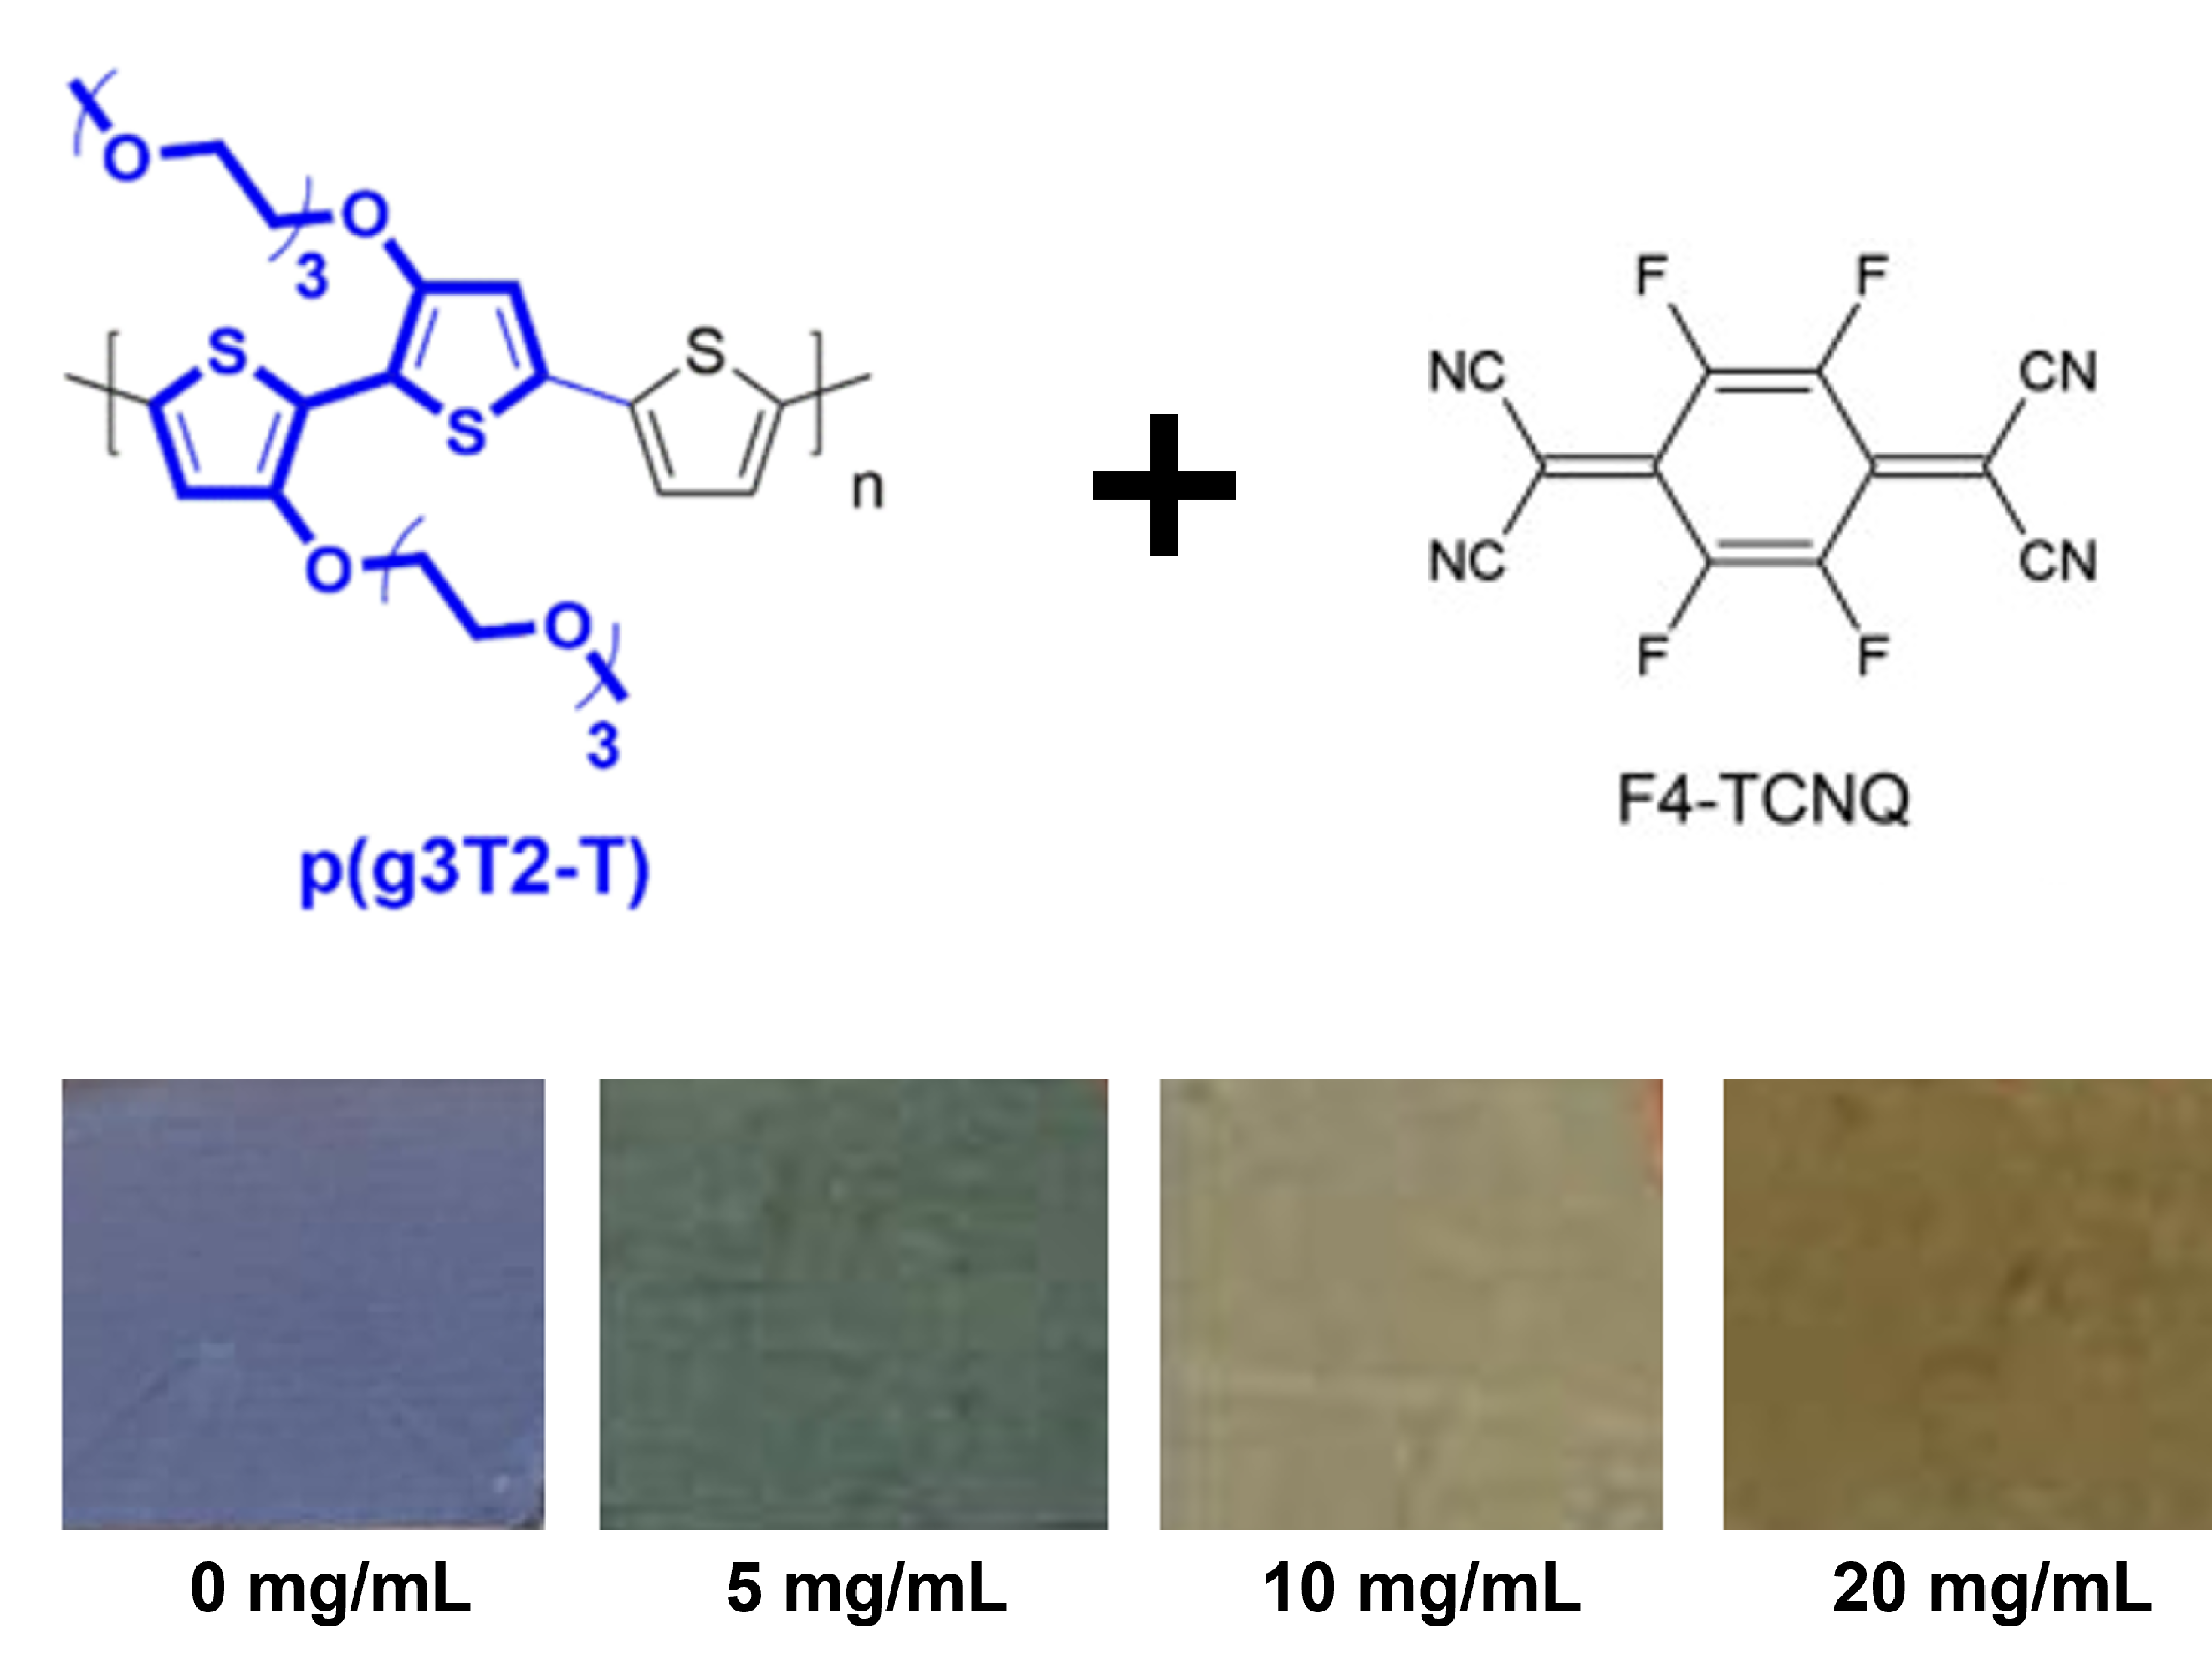
\includegraphics[width=8cm]{Images/pdf/doping_color.pdf}
  \caption[Color shift upon doping level increase]{Color change upon increasing dopant concentration from 0 to 20 mg/mL.
  \label{fig:color}}
\end{figure}

\subsection{Thickness, Sheet Resistance and Resistivity}

Sheet resistance and resistivity, as shown in Table \ref{tab:res}, were calculated using equations \ref{eq:rs} and \ref{eq:resist}, respectively, as described in previous chapter. The film thickness was determined through profilometer measurements, resulting in an approximate thickness of 70 nm.

\begin{table}[ht]
\centering
\caption{Sheet resistance and resistivity values for undoped and doped films of p(g3T2-T)}
\begin{tabular}{l|c|c|c|c}
& Undoped & 5 mg/mL & 10 mg/mL & 20 mg/mL \\\hline
R$_{S}$ ($\Omega$/sq) & 6.3M & 104.6k & 70.7k & 49.4k\\
$\rho$ ($\Omega$cm) & 44.1 & 0.73 & 0.49 & 0.35\\\hline
\end{tabular}
\label{tab:res}
\end{table}

Upon doping, a substantial decrease is observed in both sheet resistance and resistivity. However, this decrease is not as pronounced when higher dopant levels are introduced, as depicted in Figure \ref{fig:rho}. Nevertheless, when comparing the reduction among doped samples, a clear linear relationship becomes apparent with increasing the dopant concentration. 

\begin{figure}[ht]
  \centering
  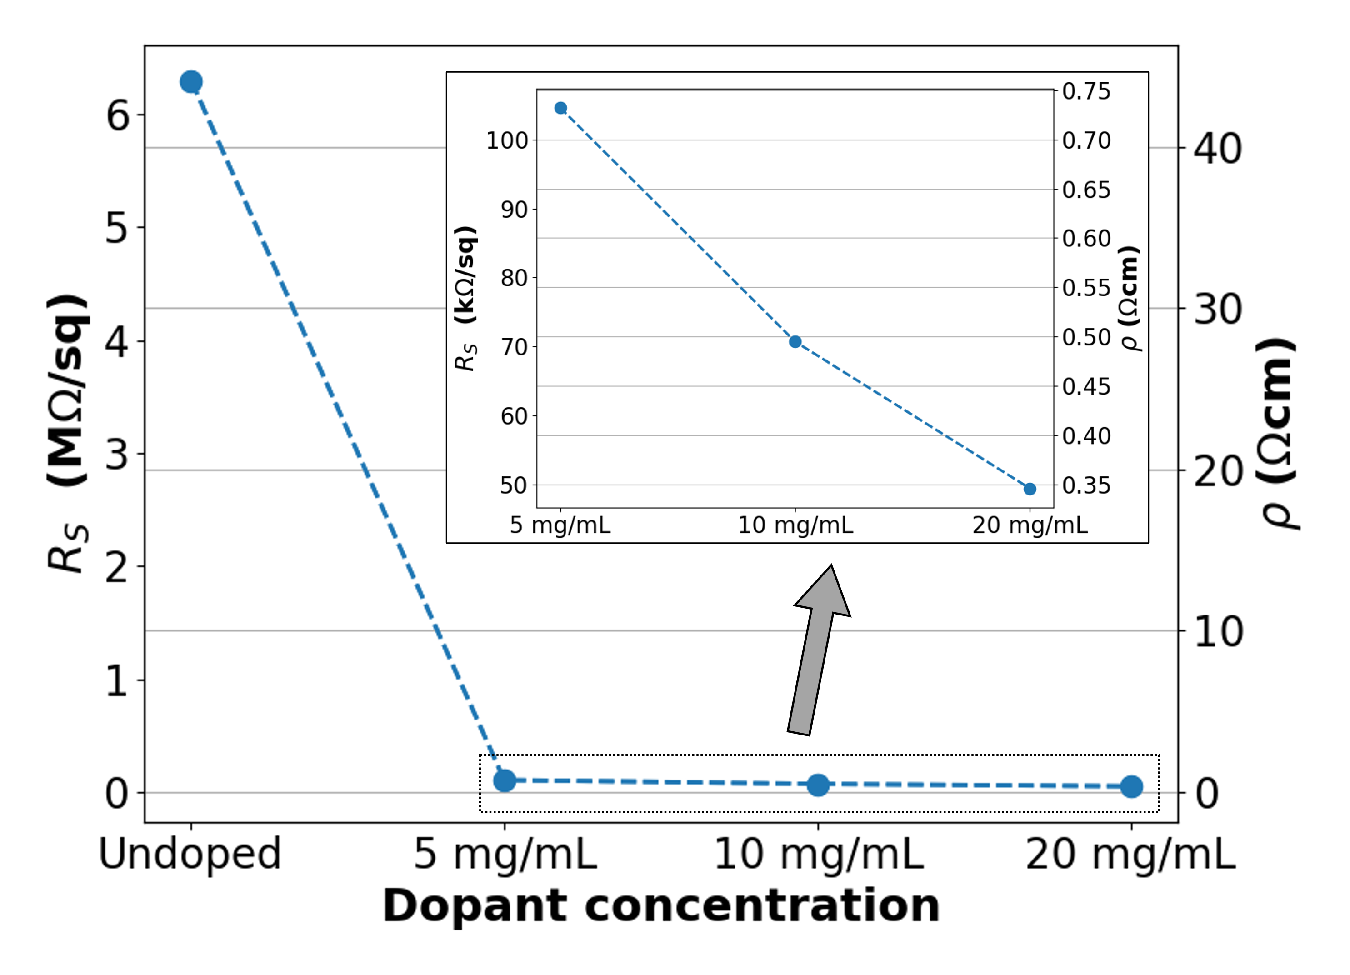
\includegraphics[width=8cm]{Images/pdf/resist+inlet.pdf}
  \caption[Sheet resistance and resistivity drop upon doping]{Sheet resistance and resistivity drop upon doping of p(g3T2-T). Inlet represents the quasi-linear drop of parameters as between doped samples.}
  \label{fig:rho}
\end{figure}

\subsection{Absorbance and Dopants Diffusion}
The visible color hue shift can be quasi-quantitatively described by examining the absorbance spectra of the samples, as illustrated in Figure \ref{fig:abs}. In the case of undoped-p(g3T2-T), there is a prominent absorption peak at 588 nm (red), which diminishes with increasing doping concentration, indicative of oxidation. Notably, new absorption peaks emerge at around 860 nm, a consequence of polaron generation, leading to new optical transitions, as explained in Chapter 2, Section \ref{subsec:moldop}. 

Tan et al. documented the appearance of new absorption peaks within the 300 to 600 nm range. The higher energy (lower wavelength) peak is generated by unreacted neutral dopant species (TCNQ$^{0}$), while the second is attributed to the new dopant anions (TCNQ$^{-}$), which induce charges in our polymer \cite{tanTuningOrganicElectrochemical2022}. Additionally, it is worth noting that, after several days of storage, the initially dominant peak of unreacted neutral dopants diminishes in intensity relative to the anions peak. This observation suggests ongoing diffusion of dopants through the polymer over time. 

\begin{figure}[ht]
  \centering
  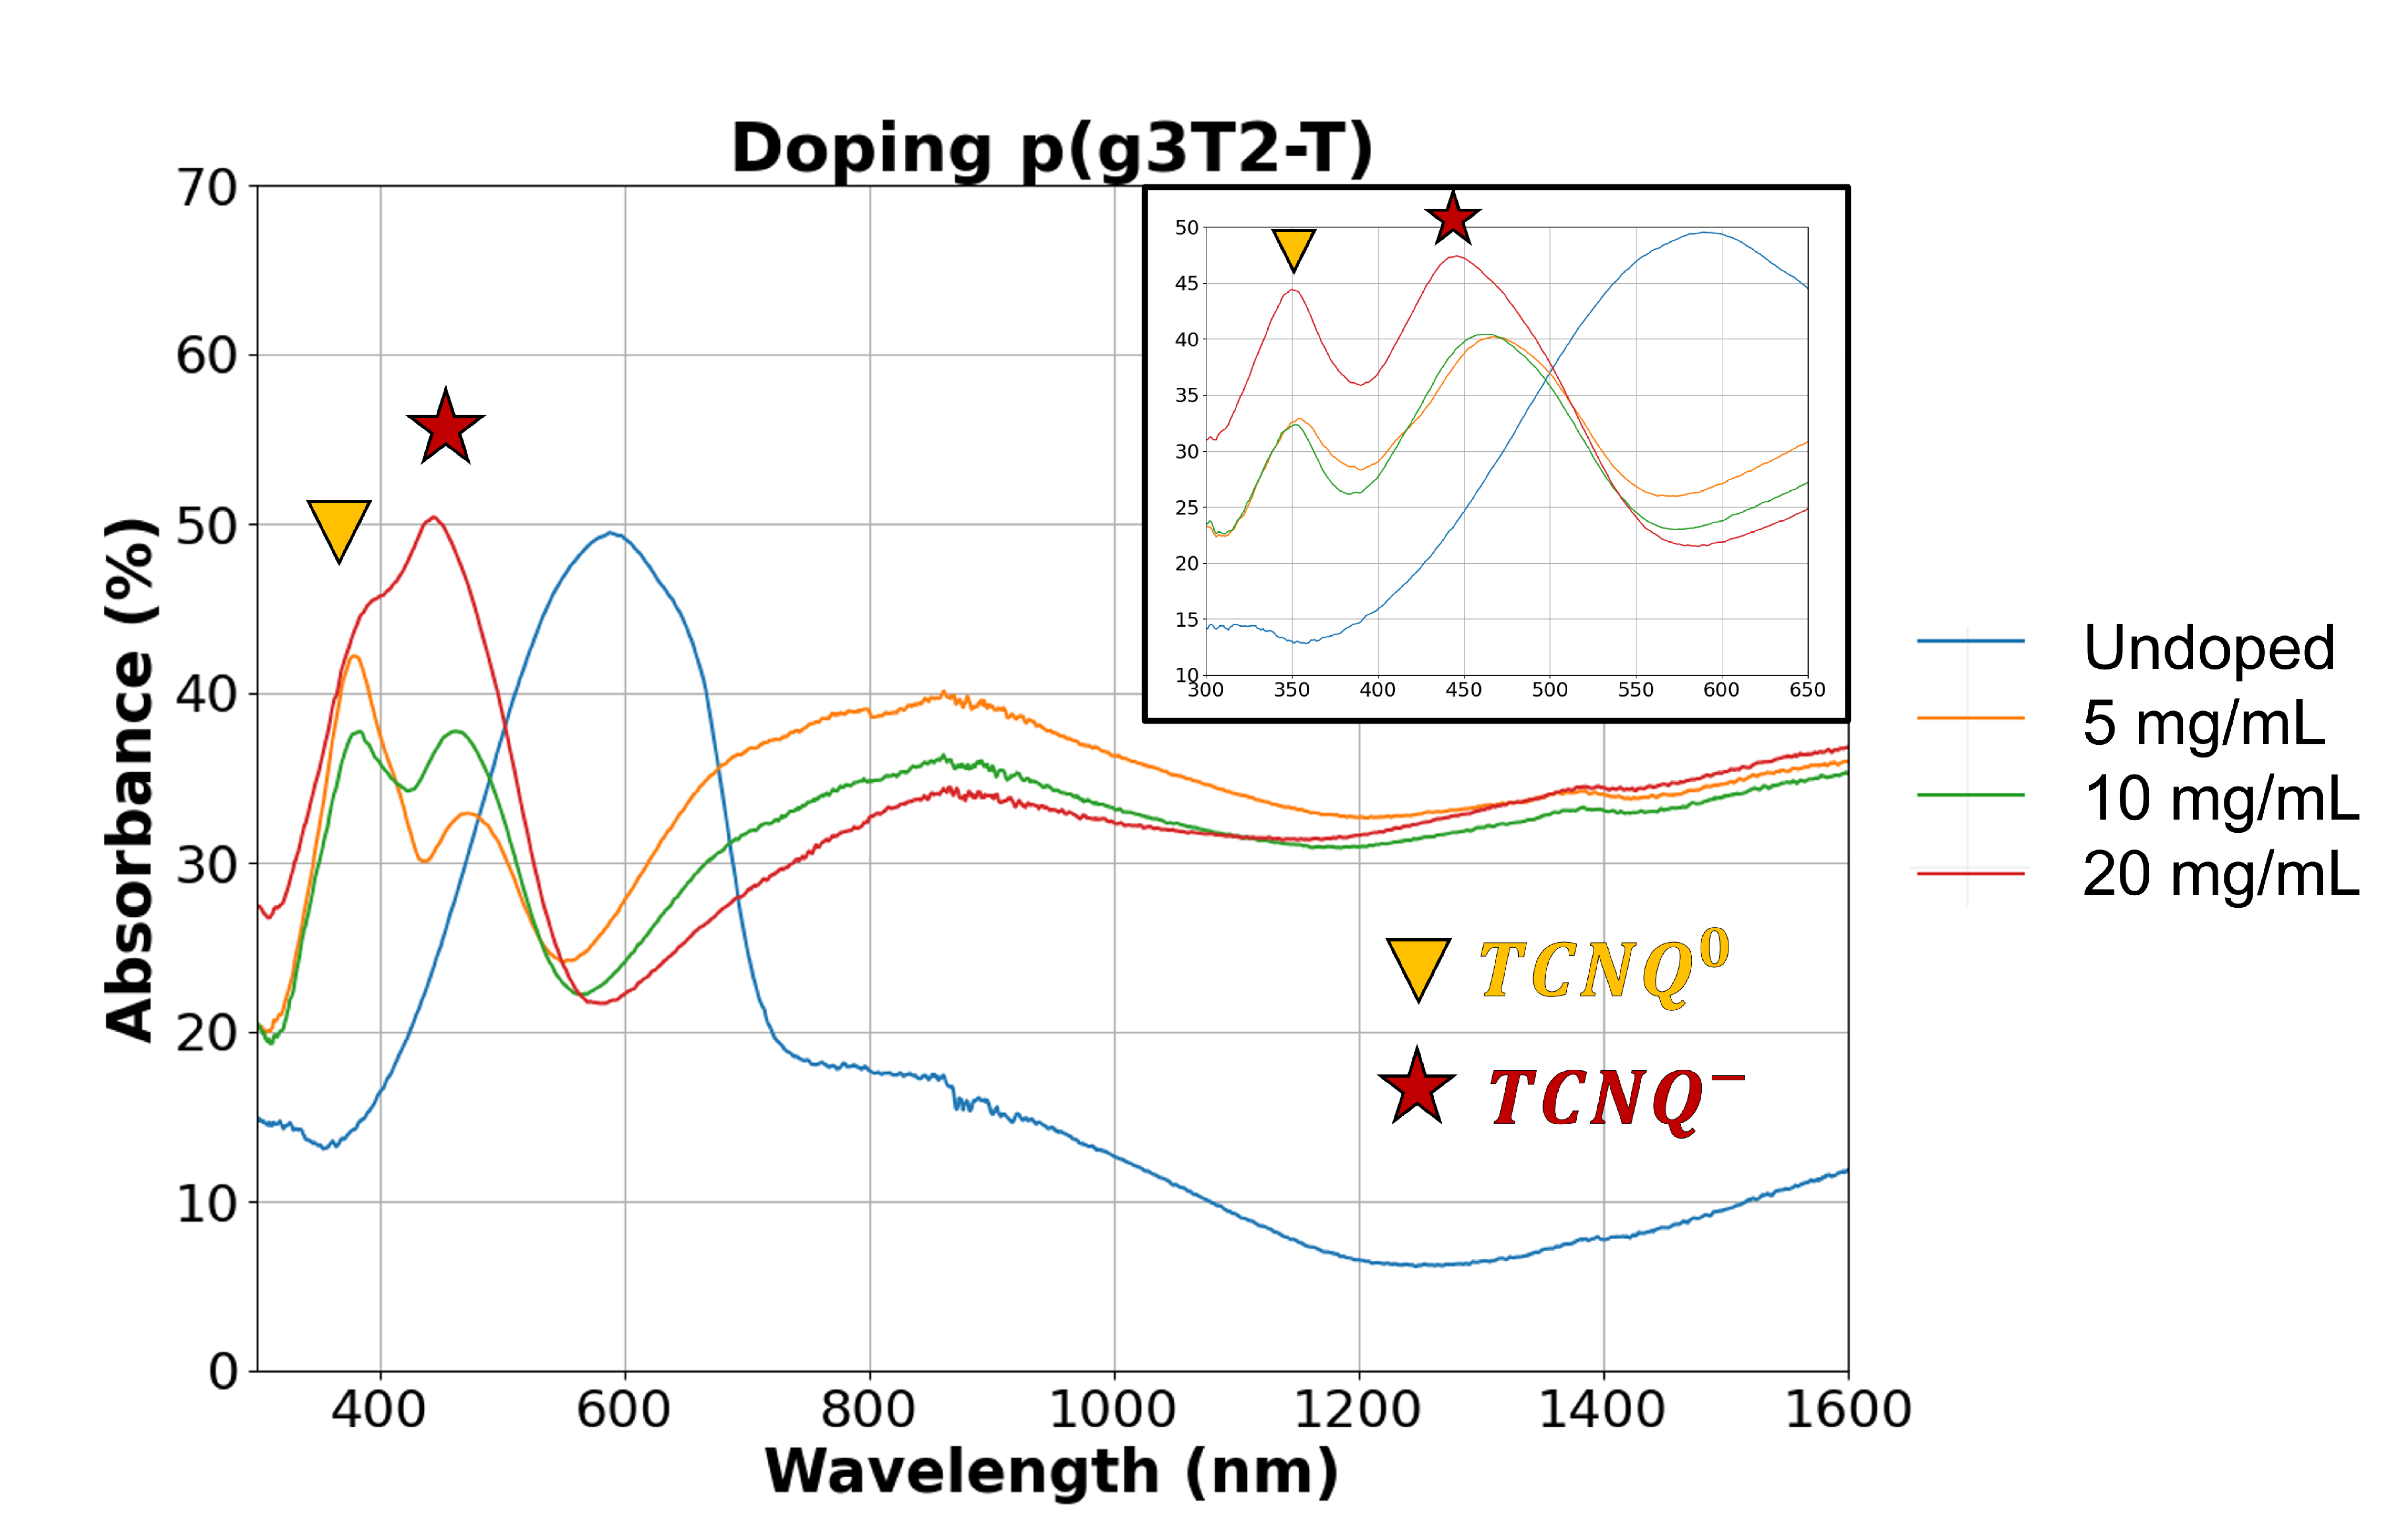
\includegraphics[width=10cm]{Images/pdf/abs+inlet.pdf}
  \caption[Absorbance spectra of different doping levels of p(g3T2-T)]{Spectra of undoped and doped-p(g3T2-T) at different doping levels, corresponding to samples on Figure \ref{fig:color}. Inlet represents absorbance after two weeks of storage in ambient conditions.}
  \label{fig:abs}
\end{figure}

Absorbance values are directly correlated with the density of states of these new optical transitions \cite{bredasPolaronsBipolaronsSolitons1985}. In our spectra, the absorbance value at 860 nm of the lowest-doped p(g3T2-T) sample (5 mg/mL) is relatively higher, around 40\%. This might initially appear counterintuitive. However, as the doping concentration increases, the formation of bipolarons and bipolaron bands becomes energetically more favorable \cite{enenglDopinginducedAbsorptionBands2016} . This phenomenon aligns with observations in the higher wavelengths, such as at 1600 nm, where absorbance increases in the more highly doped p(g3T2-T) sample.

Moreover, Tan et al. reported the formation of bipolaron in this specific context, evidenced by a shift to lower energies in the broad absorbance spectrum within the mid-IR region (wavenumbers 1000-1600 cm$^{-1}$) \cite{tanTuningOrganicElectrochemical2022}. Consequently, further analysis of hole bipolaron formation can be conducted with Fourier Transform InfraRed (FTIR) spectroscopy.
 
\subsection{Workfunction}

While the ideal preparation of films for studying electron energy levels with UPS involves working under inert conditions to prevent contamination, the current fabrication process of OECTs unavoidably exposes our films at ambient conditions. Therefore, measurements were conducted following deposition under these ambient conditions. Yet, it is possible to discern an increase in the workfunction, indicated by a shift of Fermi level of the polymer. This shift towards the HOMO level is more pronounced at higher dopant levels, as depicted in Figure \ref{fig:ups}, which is characteristic of p-type doping. Although some potential contamination prevented the measurement of samples with a dopant concentration of 20 mg/mL, the trend is clearly evident.

\begin{table}[ht]
\centering
\caption{Workfunction calculation from UPS measurements.}
\begin{tabular}{l|c|c|c}
& Undoped & 5 mg/mL & 10 mg/mL \\\hline
E$_{HBEC}$ [eV] & 17.35 & 16.47 & 16.36\\
E$_{HOMO}$ (vs E$_{F}$) & 4.28 & 3.27 & 3.24\\
WF [eV] & 3.87 & 4.28 & 4.86\\\hline
\end{tabular}
\label{tab:ups}
\end{table}

It is important to consider that UPS is a surface-sensitive measurement. The penetration depth of the ultraviolet-range electrons in UPS is approximately 2 nm, significantly less than our polymer thickness (approximately 70 nm). Consequently, this technique constrains our understanding of the diffusion of dopants throughout the entire volume of the polymer. While, we gained some insights into this matter in the previous subsection, further analysis could be undertaken using X-Ray Photoelectron Spectroscopy which offers a depth profiling mode. %but along with depth profiling mode 3

\begin{figure}[ht]
	\centering
	\subfloat[]{{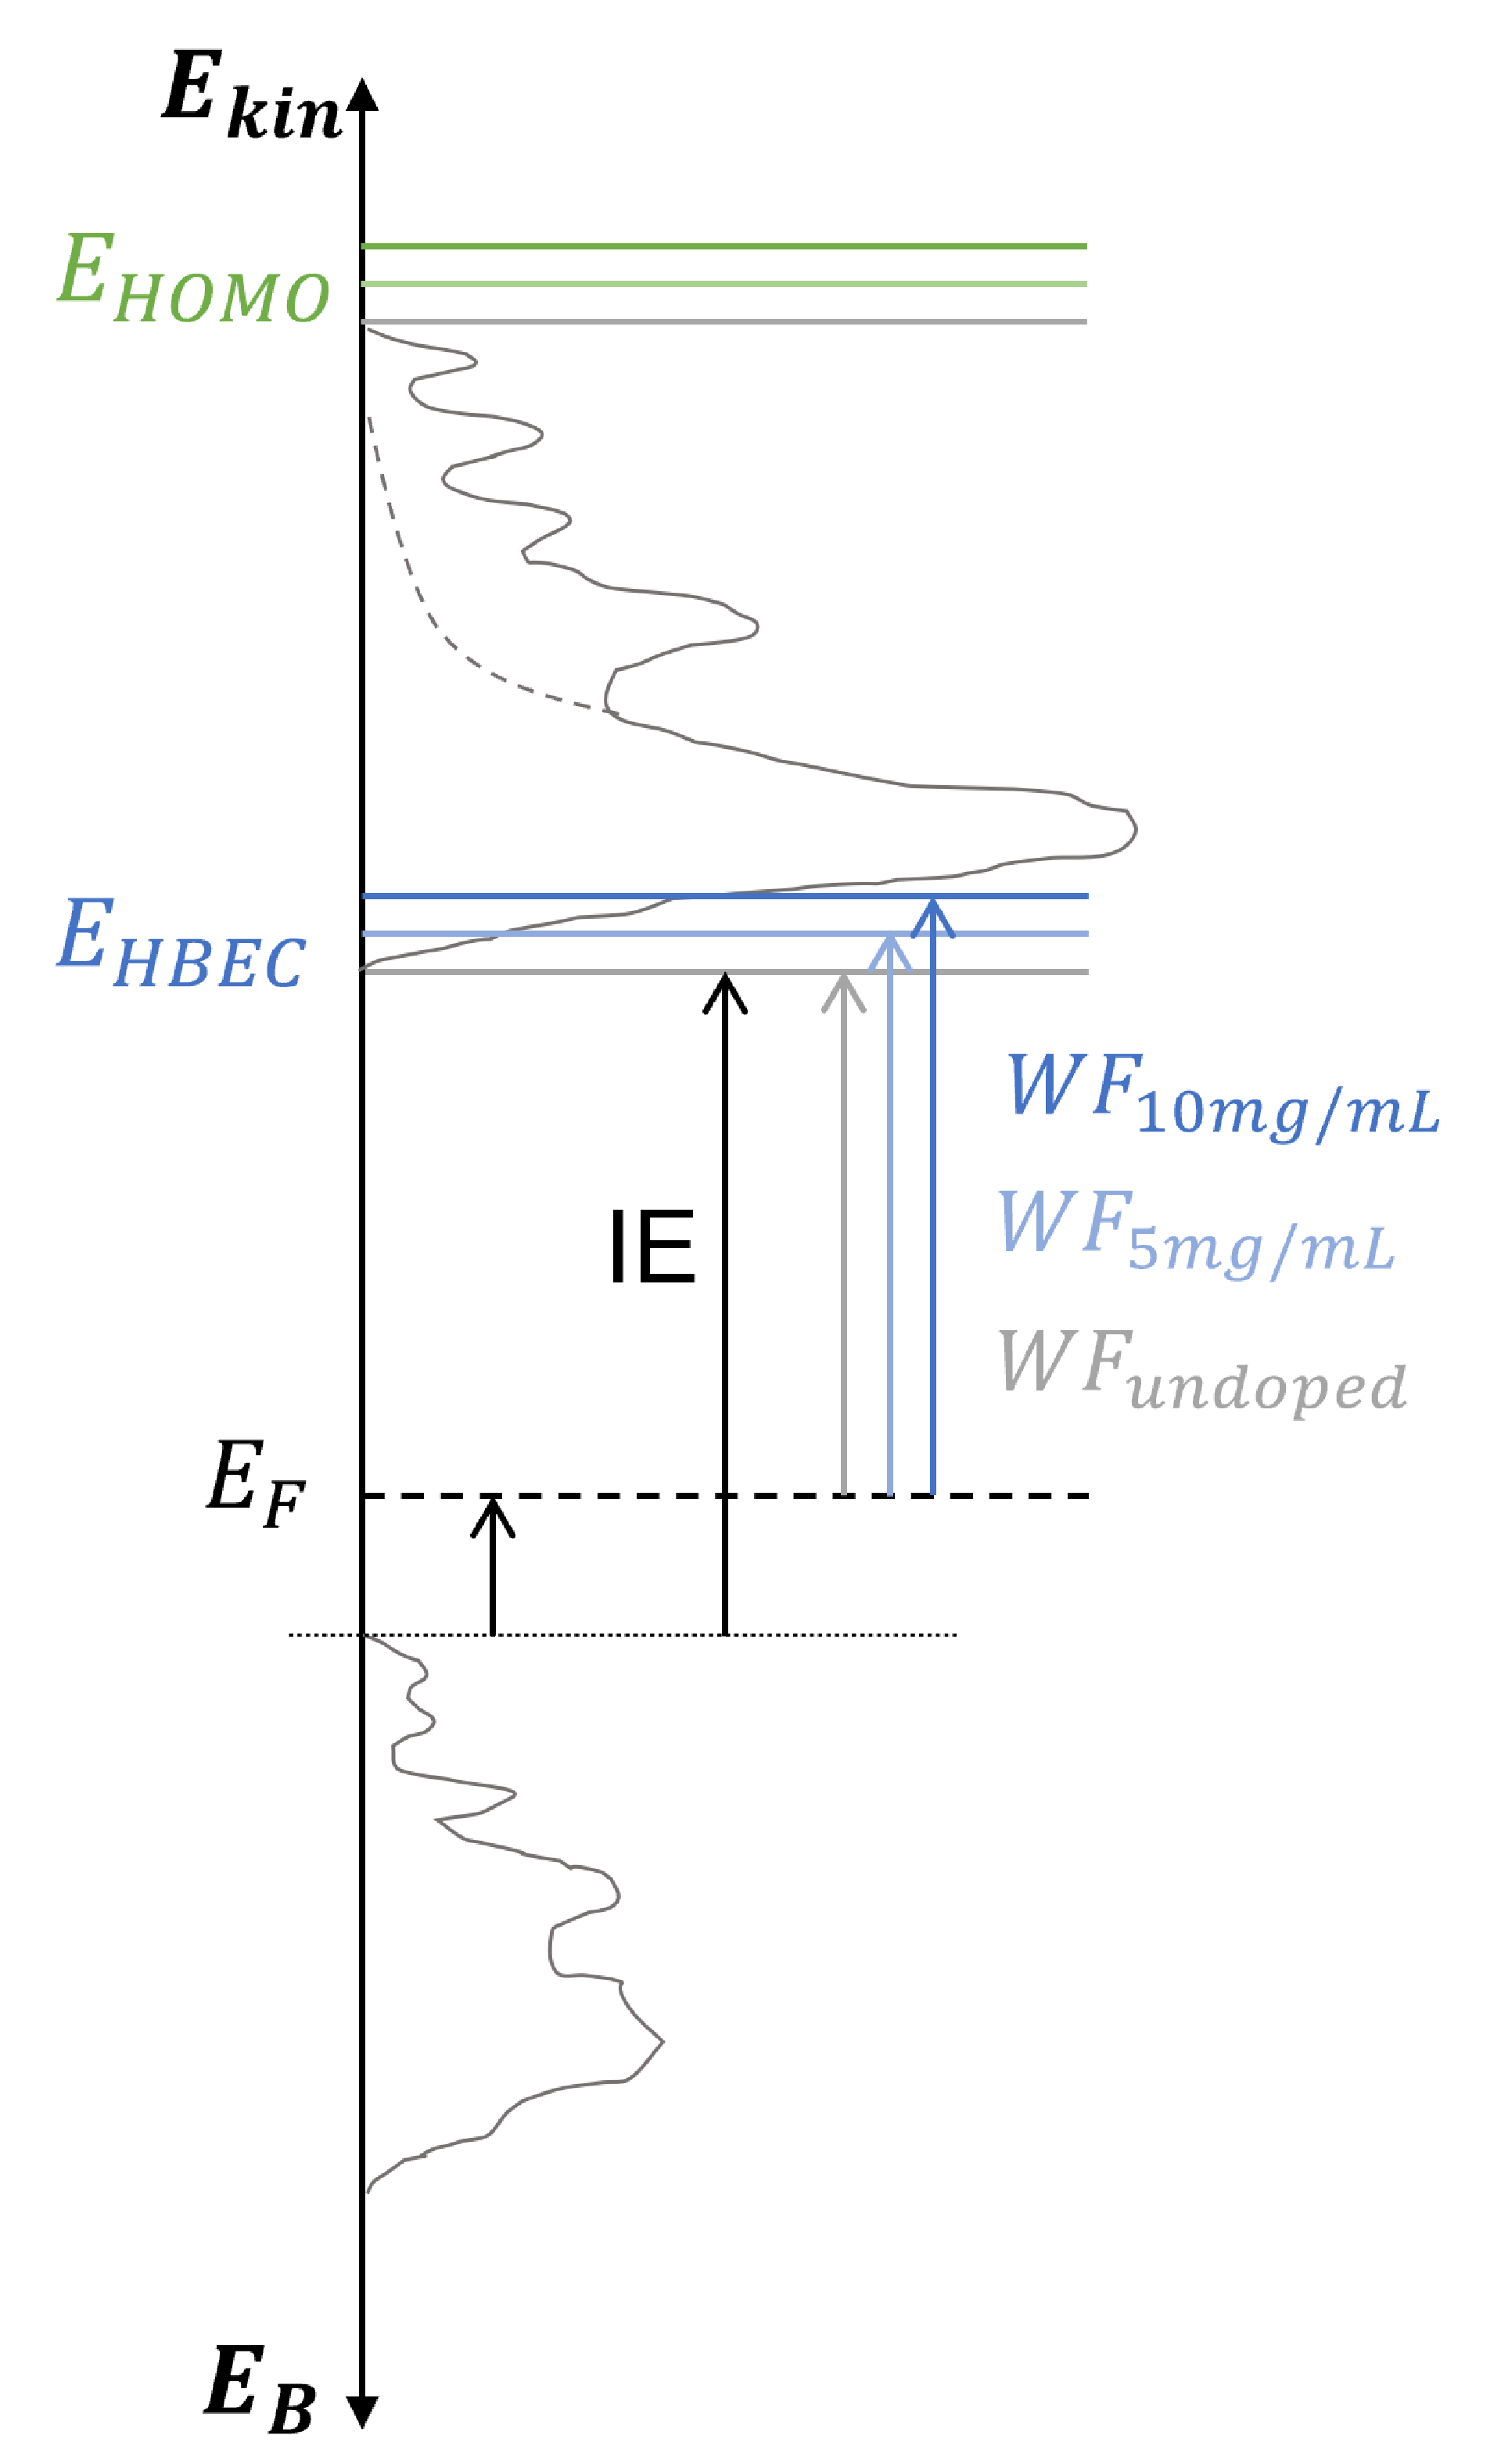
\includegraphics[width=6cm]{Images/pdf/WF_final.pdf} }}
	%\qquad
	\hspace{2em}
	\subfloat[]{{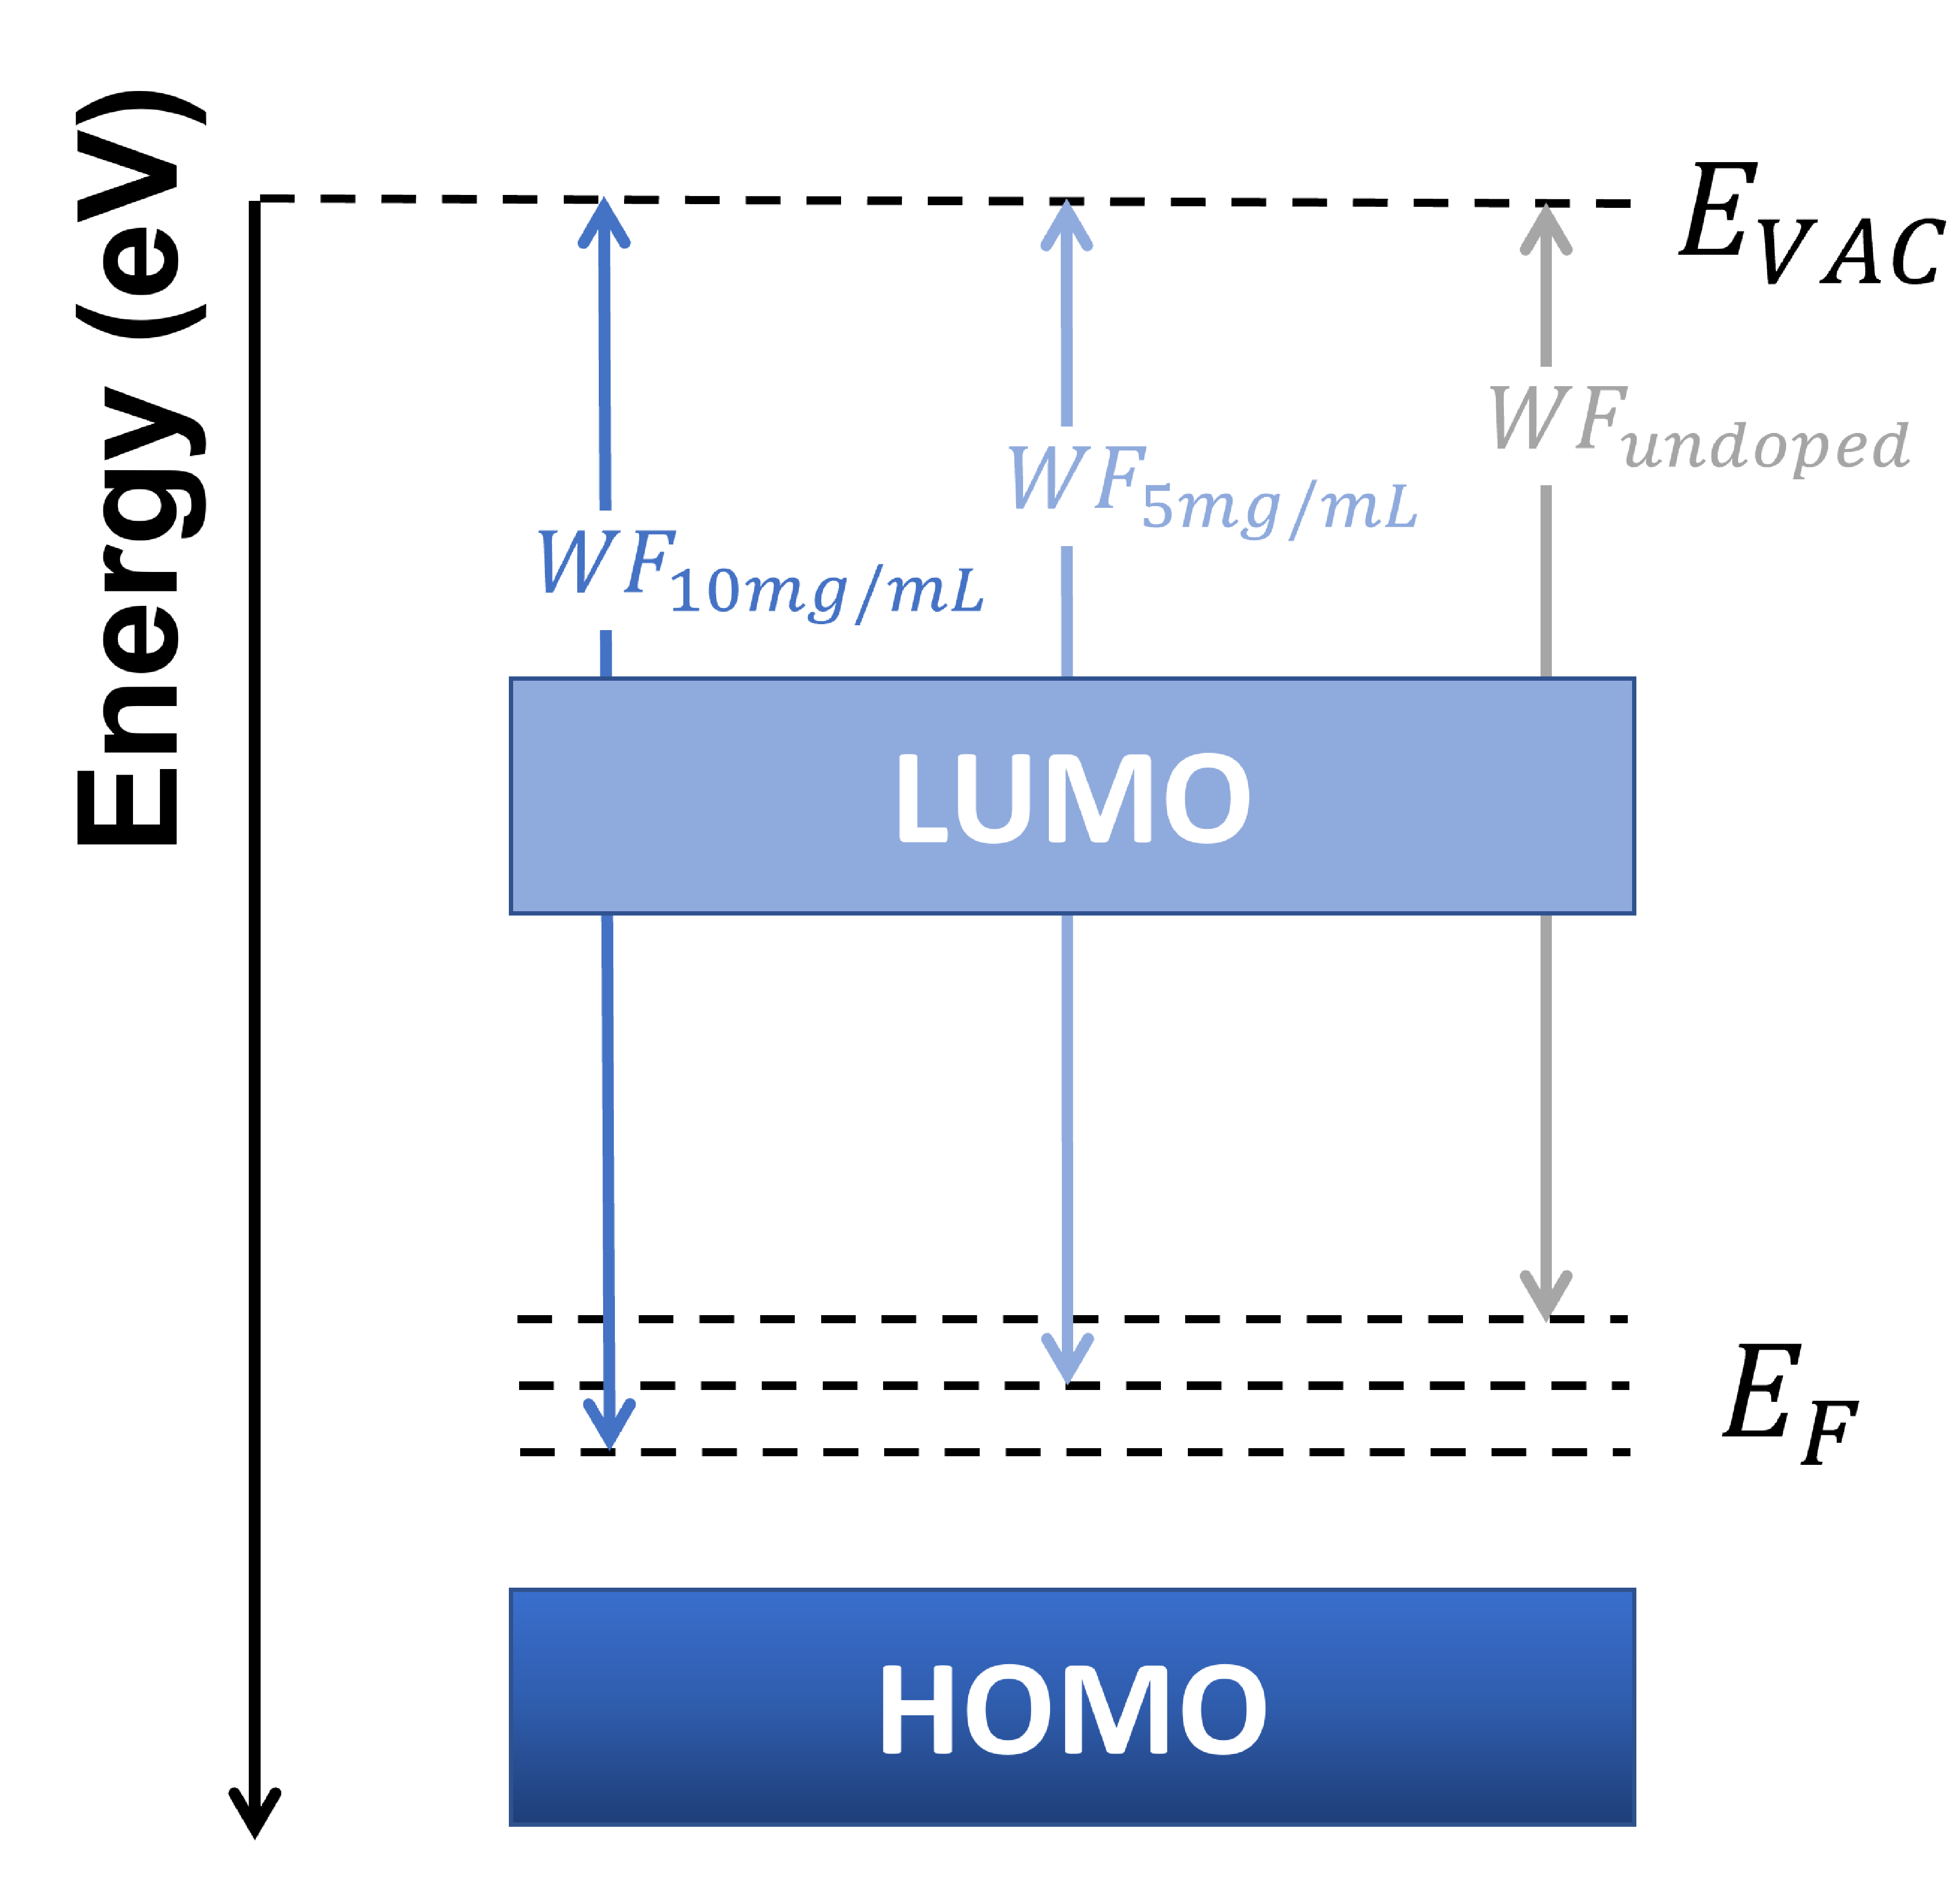
\includegraphics[width=6.5cm]{Images/pdf/WF.pdf} }}
	\caption[Representation of the Fermi level shift upon doping]{ Graphical representation of A) the relationship between the binding energies E$_{B}$ and the kinetic energy of the photoelectrons E$_{kin}$, and B) the Fermi level shift, upon doping.} 
	\label{fig:ups}
\end{figure}

%\subsection{Roughness}

\section{Fabrication of Organic Electrochemical Transistors}
The patterning process was successfully achieved with photolithography by using a mask that include a microstructure gate, suitable for studying OECTs with both channel and gate made of the same OMIEC material, commonly PEDOT:PSS. The result is displayed in Figure \ref{fig:channel}. 

\begin{figure}[ht]
  \centering
  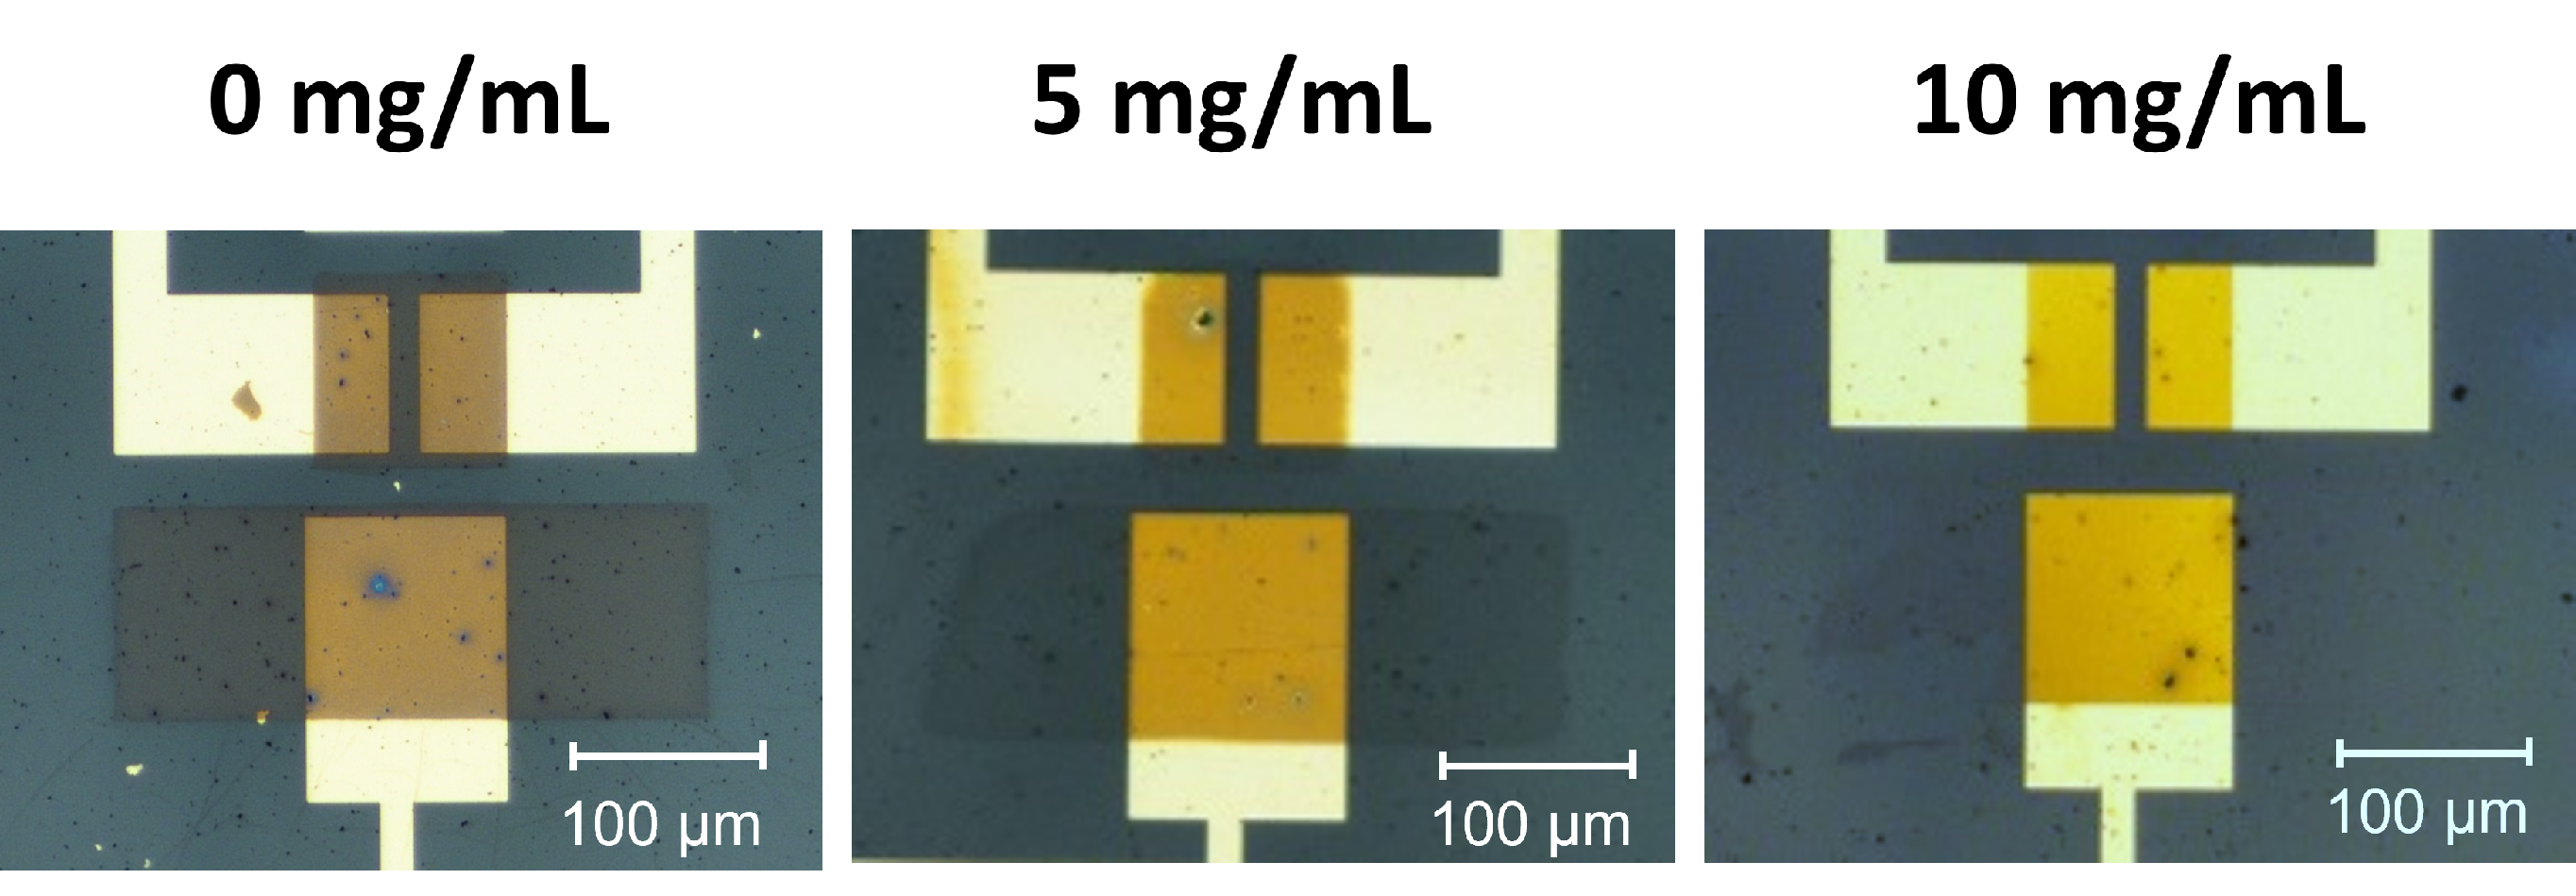
\includegraphics[width=10cm]{Images/pdf/BigGateDevices.pdf}
  \caption[Micrographs of a patterned channel and gate p(g3T2-T) at different doping levels]{Micrographs of patterned channel and gate with p(g3T2-T) undoped, 5 mg/mL and 10 mg/mL dopants, following procedures explained in Section \label{subsec:photo}.}
  \label{fig:channel}
\end{figure}

%Prior biasing gate, which is due to passive (ion) diffusion?

\subsection{Influence of Doping on OECT Channel}
Since our final goal is to study fully patterned solid-OECTs that will allow integrated circuits (IC), which was not reported in the literature for this material. It was necessary to first understand the solely impact of the channel doping in our devices. Some hypothesis comes along, based on reference \cite{tanTuningOrganicElectrochemical2022}:

\begin{enumerate}
\item The manipulation of channel doping will negatively impact transfer characteristics.
\item The introduction of ionic species (TCNQ$^{-}$) in p(g3T2-T) should create depletion-mode devices with positive threshold voltages. Since a higher positive gate biased would be needed to counteract these anions and turn OFF the device.
\end{enumerate}

As explained in the last chapter, we paired our channel with a non-polarizable Ag/AgCl electrode as gate, and coupled with SSE precursor. Unfortunately, the sample that used solution with dopant concentration of 20 mg/mL exhibited doping homogeneity issues. While photolithography was still possible, it could not provide a fair basis for comparison with the other devices. Therefore, this sample will be omitted from this analysis.

The results shown in Figure \ref{fig:transx2}, Figure \ref{fig:shift1} and Figure \ref{fig:vth_vds} correspond to the same device and same loop on each sample (undoped, 5 mg/mL and 10 mg/mL dopants) from the same batch of materials. After reporting the findings on the analysis of these devices, a more statistical study will be shown within the operating devices on each sample. An important consideration for the statistical analysis of this part is that besides the attempts to increase the yields, only 3 or 4 out of the 14 devices were operational on each sample. Further improvements on the photolithograpy process were needed, and were accomplished as it will be shown in further sections of this chapter. 

Transfer characteristics are illustrated in Figure \ref{fig:transx2}A, C, E which correspond to undoped, 5 mg/mL and 10 mg/mL dopants, respectively. A positive turn ON voltage is perceived in the undoped OECT device, which evidenced the fast oxidation (unwanted doping) of p(g3T2-T) under environmental conditions due to its low IP. 

The drain current ($I_{D}$) of the undoped device shows higher values than doped devices, Hidalgo et al. reported that pristine p(g3T2-T) show oxygen reduction reaction activity in oxygen-saturated conditions, therefore, it is expected an increase of current within the polymer until saturation \cite{hidalgocastilloSimultaneousPerformanceStability2022a}. It will be necessary to control the oxidation state of the polymer among the different steps of the photolithography process, or somehow revert the oxidation of p(g3T2-T), this will be addressed in the following sections.

Gate current ($I_{G}$) is displayed in dotted lines and it is perceived that the drain OFF current ($I_{D,OFF}$) is dominated by this leakage current in all devices. %Figure \ref{fig:shift1} shows doped devices have minimum differences on $I_{D,OFF}$.

The higher dopant concentration device (10 mg/mL dopant) shows signs of breakage as going to more negative $V_{DS}$ (Figure \ref{fig:transx2}E and Figure \ref{fig:shift1}D), therefore, this measurement will be disregard for calculating transconductance and threshold voltage.

\begin{figure}[!htb]
    \centering
    \subfloat[Undoped device]{{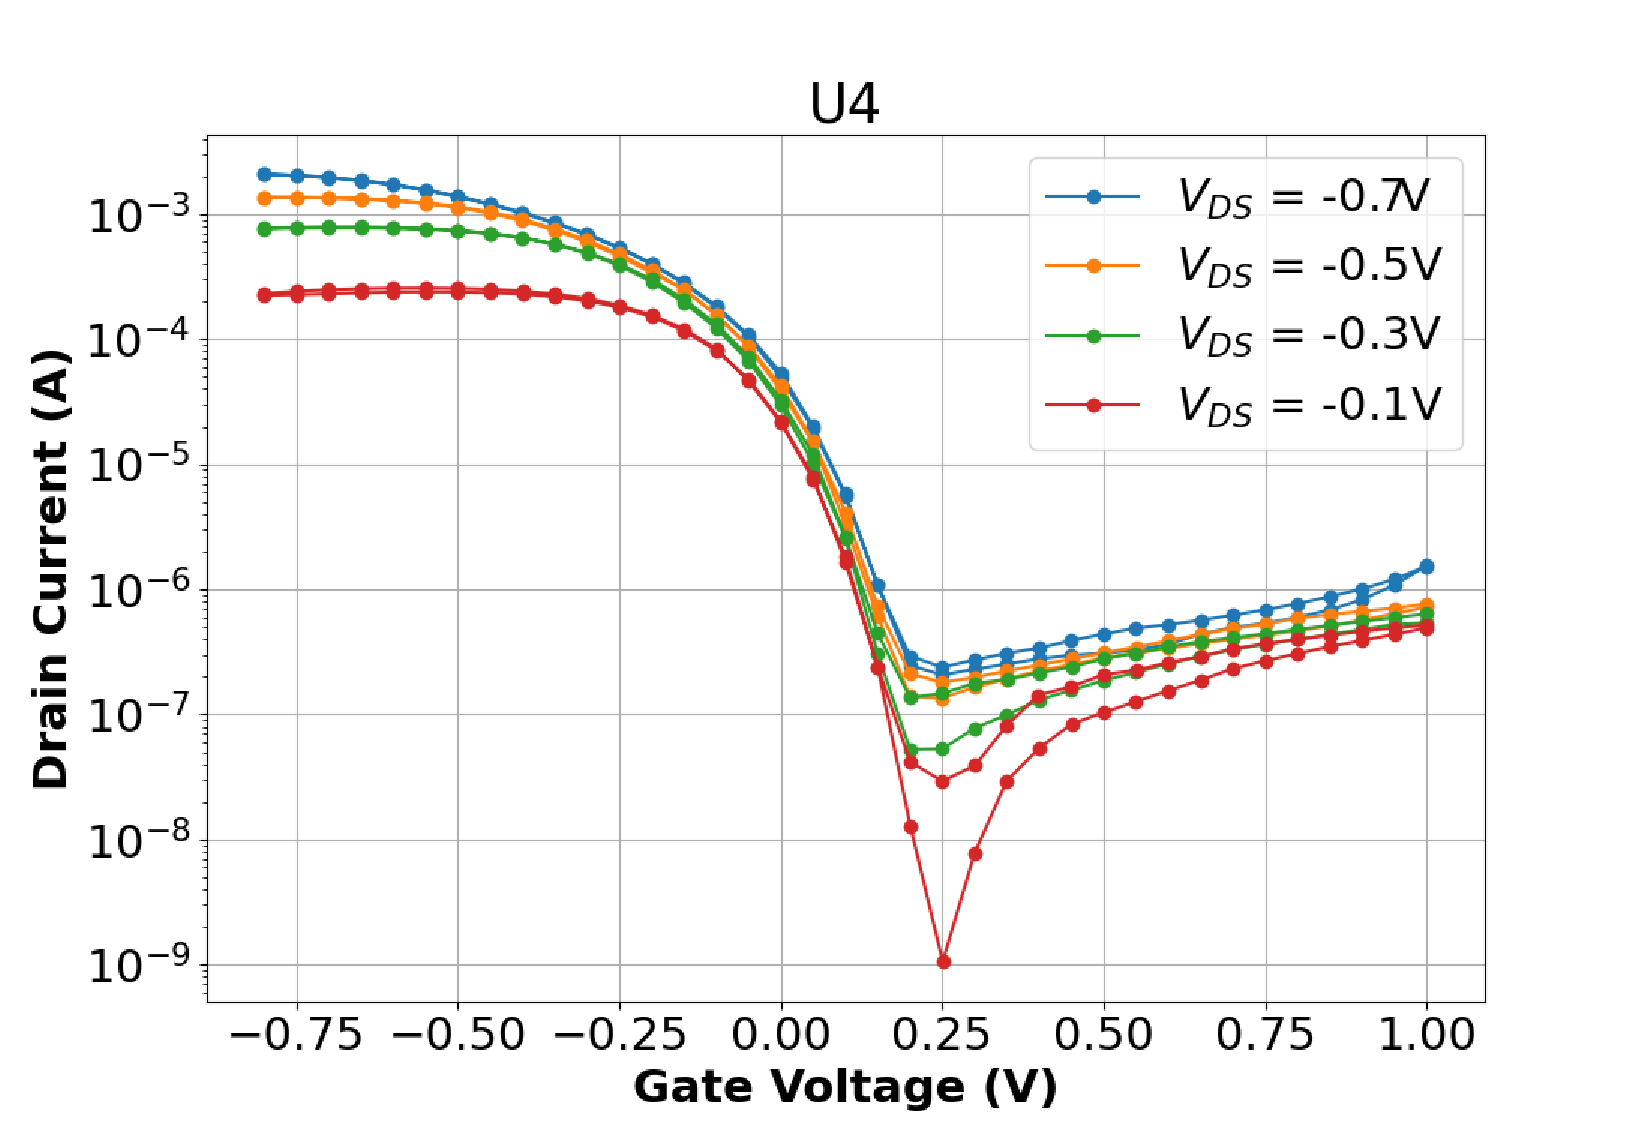
\includegraphics[width=5.7cm]{Images/pdf/transfer_undoped.pdf} }}
    \subfloat[Undoped device]{{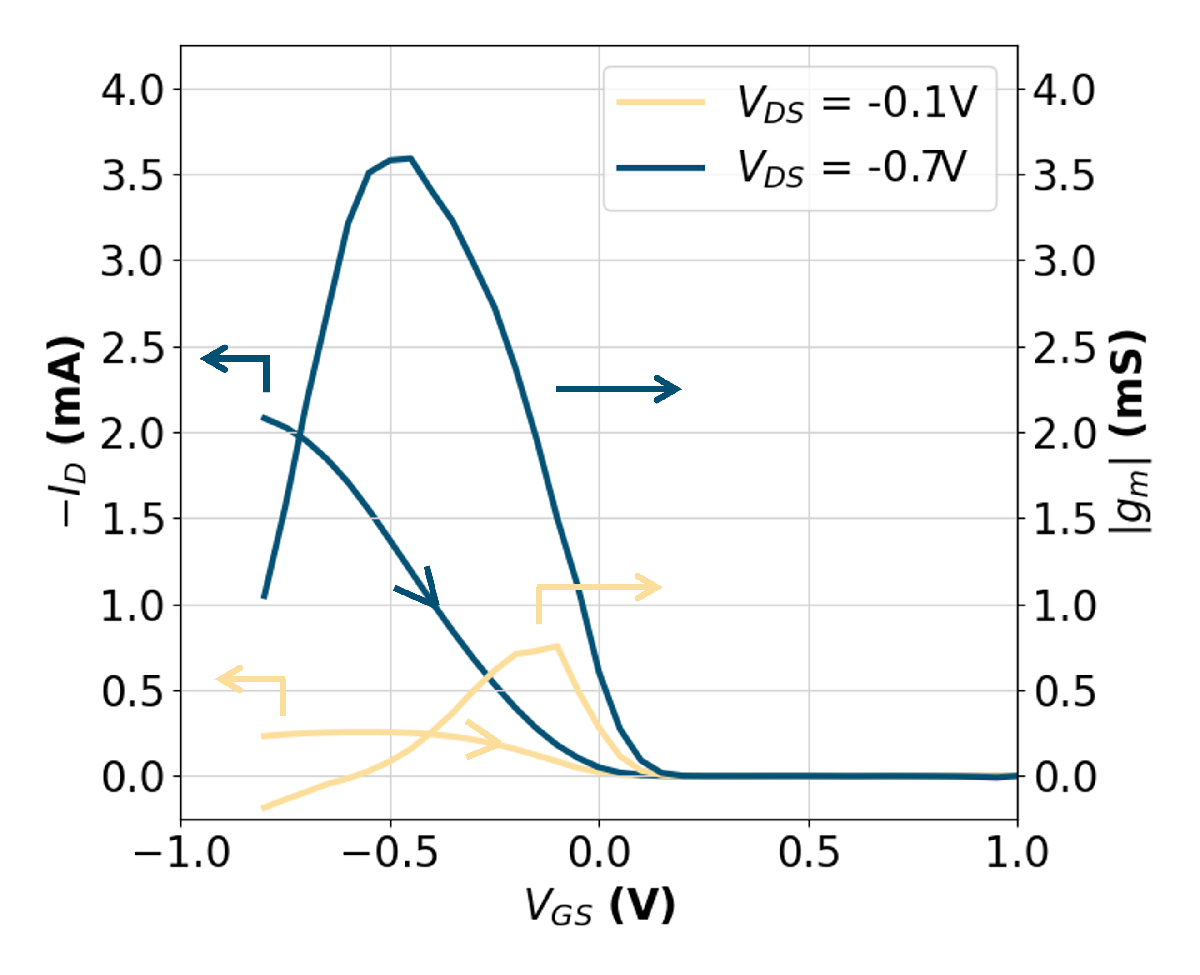
\includegraphics[width=5.3cm]{Images/pdf/id+gm_undoped_final.pdf} }}
    \qquad
    \subfloat[5 mg/mL dopant device]{{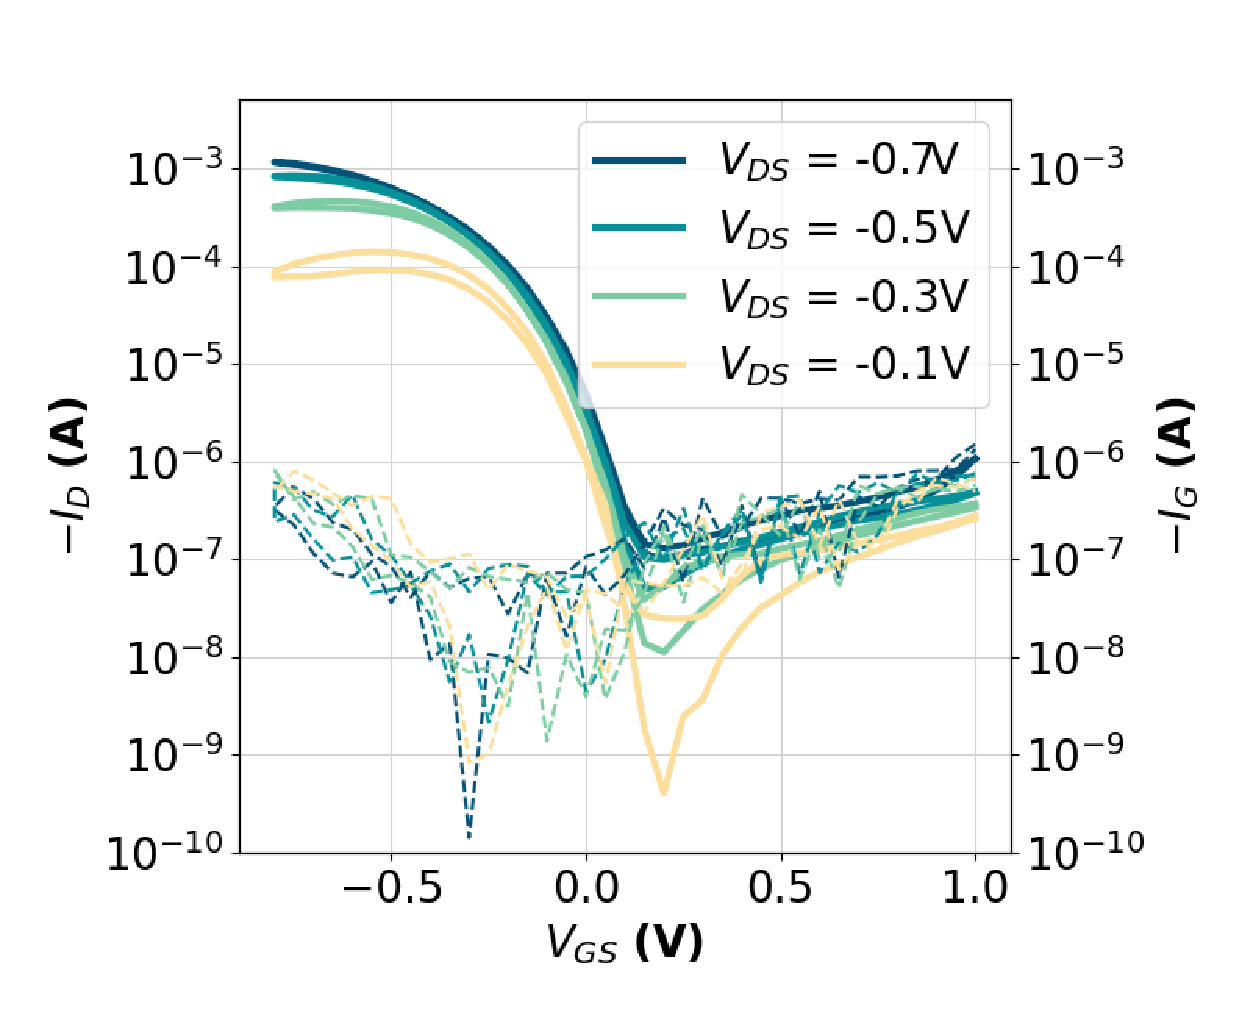
\includegraphics[width=5.7cm]{Images/pdf/transfer_doped5.pdf} }}
    \subfloat[5 mg/mL dopant device]{{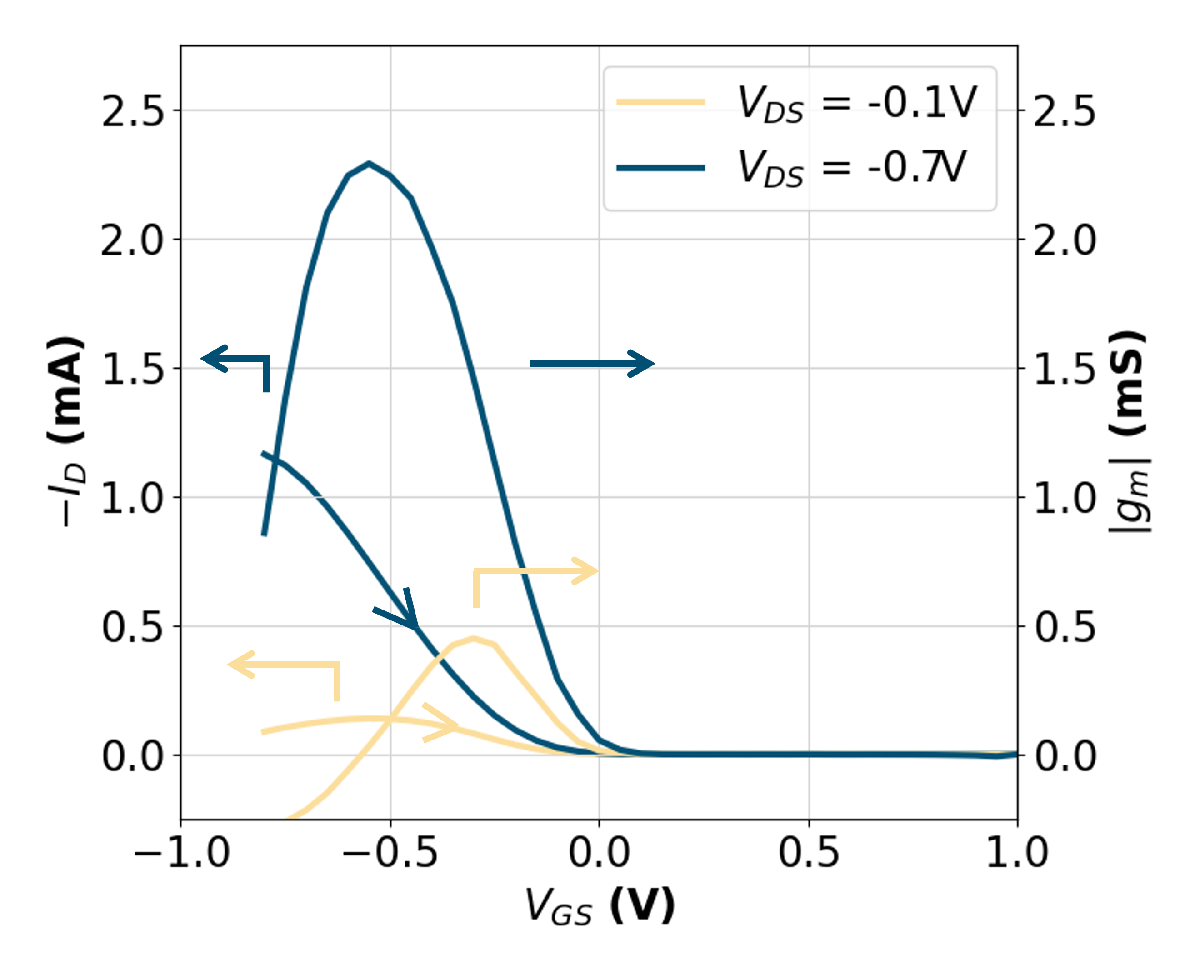
\includegraphics[width=5.3cm]{Images/pdf/id+gm_doped5_final.pdf} }}
    \qquad
    \subfloat[10 mg/mL dopant device]{{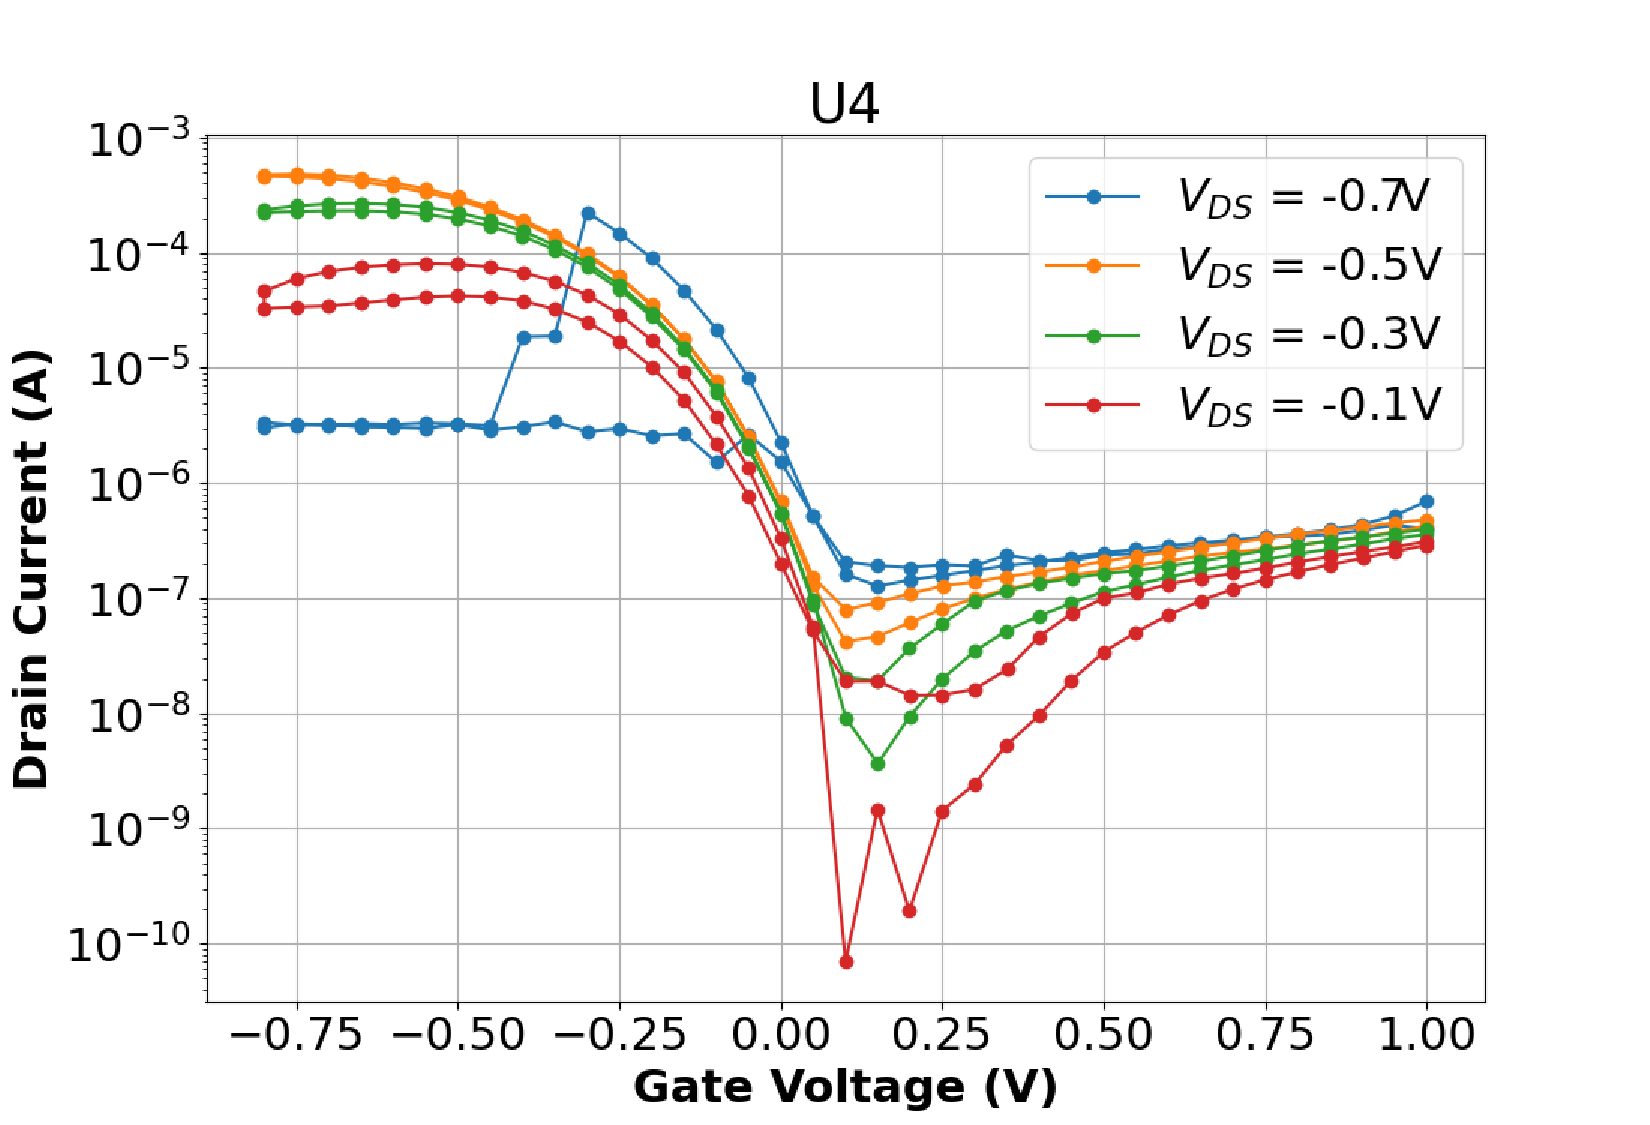
\includegraphics[width=5.7cm]{Images/pdf/transfer_doped10.pdf} }}
    \subfloat[10 mg/mL dopant device]{{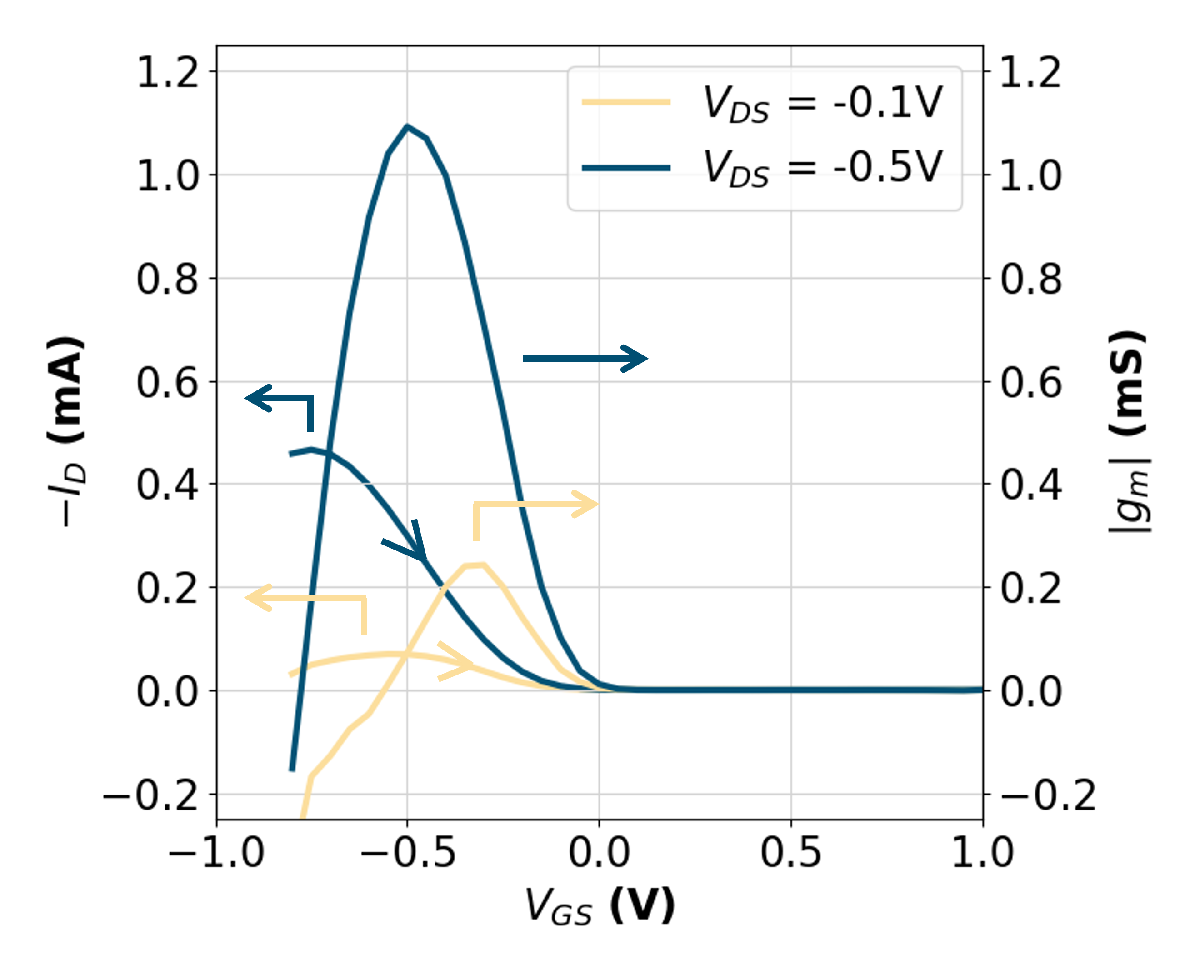
\includegraphics[width=5.3cm]{Images/pdf/id+gm_doped10_final.pdf} }}
    \caption[Transfer characteristics and transconductance at different doping levels and $V_{DS}$]{A), C), E) Transfer characteristics of all measured $V_{DS}$ including the gate leakage current $I_{G}$ B), D), F) Transfer curves (off-switching) with corresponding transconductance. Each group of graphs for undoped, 5 mg/mL and 10 mg/mL doped p(g3T2-T) channel, respectively.}
    \label{fig:transx2}
\end{figure}

%U4 loop 2 as undoped pattern
%U2 loop 3 for doped 5
%U4 loop 3 for doped 10

In Figure \ref{fig:shift1}, it can be perceived that doped devices exhibit minimum differences on $I_{D,OFF}$ but $I_{D,ON}$ decreases while increasing doping levels. This is reflected in the maximum transconductance values displayed in Table \ref{tab:trans}, a clear drop of |$g_{m,max}$| is seen as doping level increases. From our initial hypothesis, this was expected and a further analysis will be performed later with impedance measurements to calculate volumetric capacitance. %, since as explained in the Background chapter, Section \ref{subsec:devphy}, $I_{D}$ depends on this values along with the charge carrier mobility.

%When doping our polymer, we are increasing its conductivity by inducing new charges in its backbone, however, the introduction of new ionic species will negatively impact the mobility of the induced charges, which explains the decrease in $I_{D,ON}$. %????

\begin{table}[ht]
\centering
\caption{Maximum transconductance values extracted from Figure \ref{fig:transx2}B, D, F}
\begin{tabular}{l|c|c|c}
|g$_{m,max}$| [mS] @ & Undoped & 5 mg/mL & 10 mg/mL \\\hline
$V_{DS}$ = -0.1 V & 0.75 & 0.45 & 0.24\\
$V_{DS}$ = -0.3 V & 2.01 & 1.31 & 0.74\\
$V_{DS}$ = -0.5 V & 2.90 & 1.97 & 1.09\\
$V_{DS}$ = -0.7 V & 3.59 & 2.23 & \\ \hline
\end{tabular}
\label{tab:trans}
\end{table}

More importantly and what caught our attention, results displayed in Figure \ref{fig:shift1} and Figure \ref{fig:vth_vds} evidenced turn ON voltages and threshold voltages, respectively, \textbf{shifted towards negative values} as the dopant concentration increased in all $V_{DS}$ values, \textbf{contradicting our initial hypothesis}. A sort of \textbf{compensation doping effect} is evidenced in the OECTs. Further investigation is needed to counteract this effect. %, and as explained in the Background chapter, p(g3T2-T) as a type VI OMIEC, unlike PEDOT:PSS, have ionic species as free carriers and not chemically bonded. Further analysis in the conductivity needs to be done to understand to impact of this coupling in our undoped and doped polymer.
%% EG3 ensure no cation trapping in the crystalline phase of OMIECs

\begin{figure}[ht]
    \centering
    \subfloat[$V_{DS}$ = -0.1 V]{{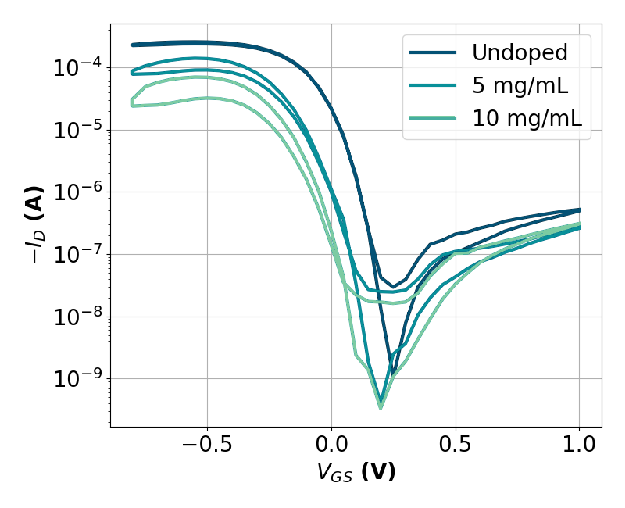
\includegraphics[width=5.5cm]{Images/pdf/Shift_Vds1.pdf} }}
    \subfloat[$V_{DS}$ = -0.3 V]{{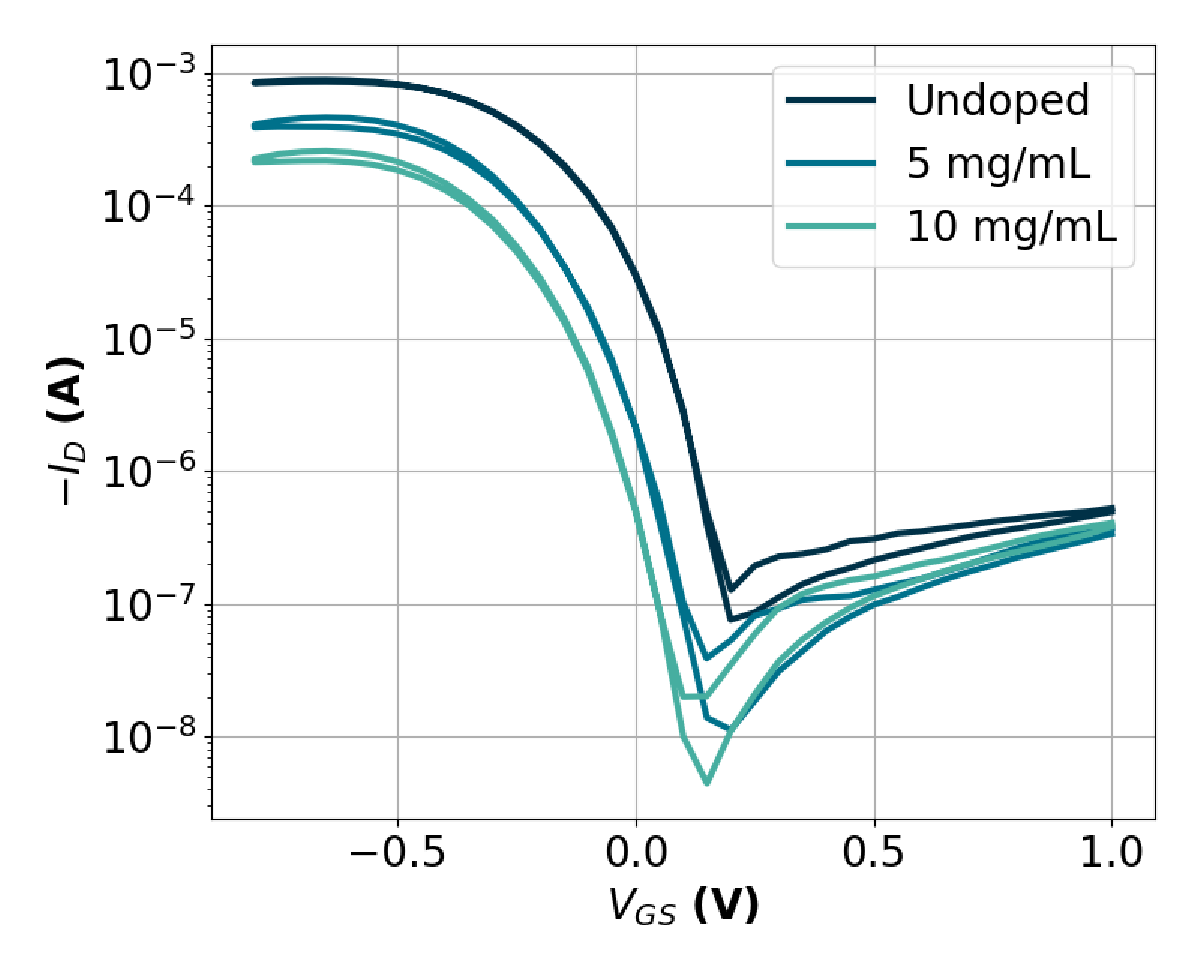
\includegraphics[width=5.5cm]{Images/pdf/Shift_Vds3.pdf} }}
    \qquad
    \subfloat[$V_{DS}$ = -0.5 V]{{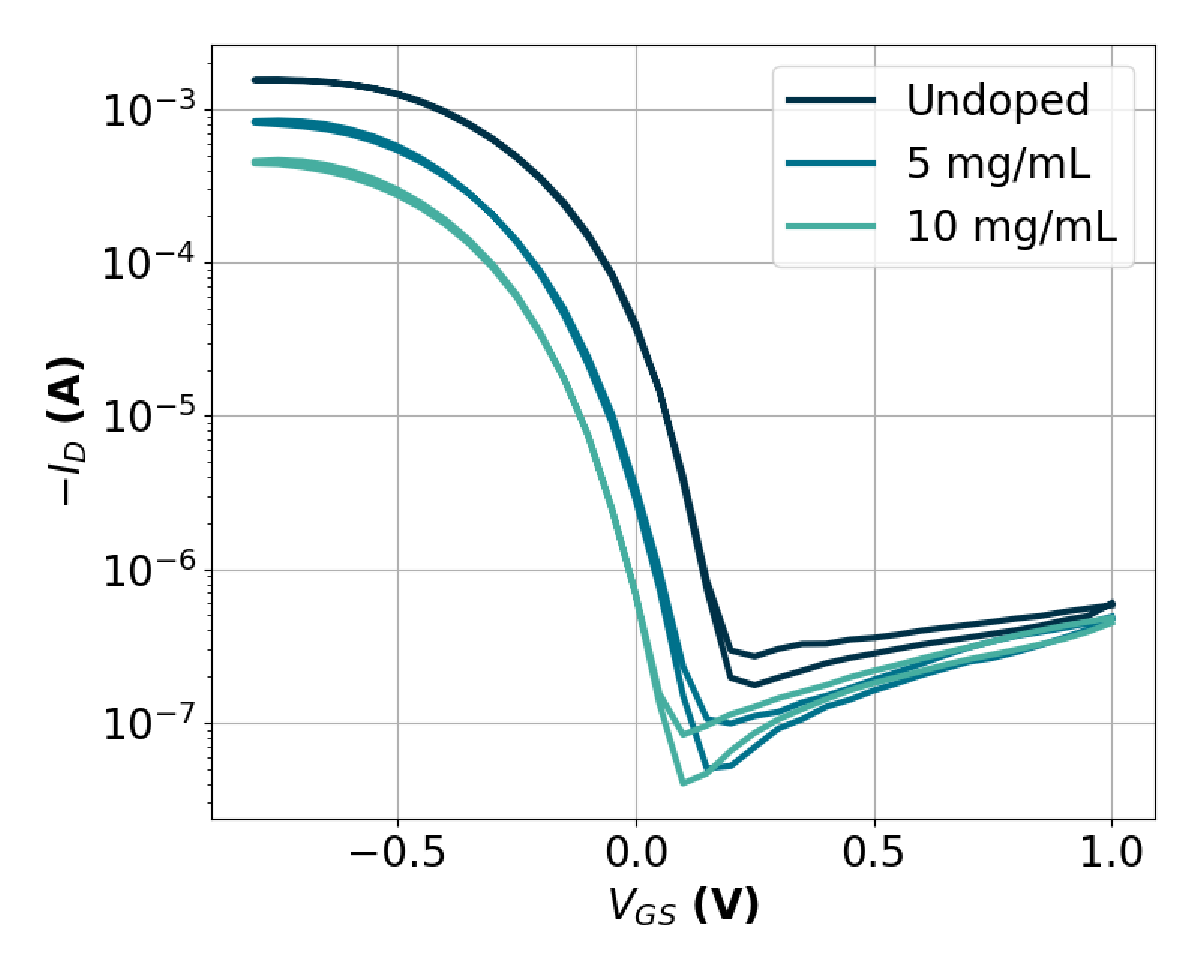
\includegraphics[width=5.5cm]{Images/pdf/Shift_Vds5.pdf} }}
    \subfloat[$V_{DS}$ = -0.7 V]{{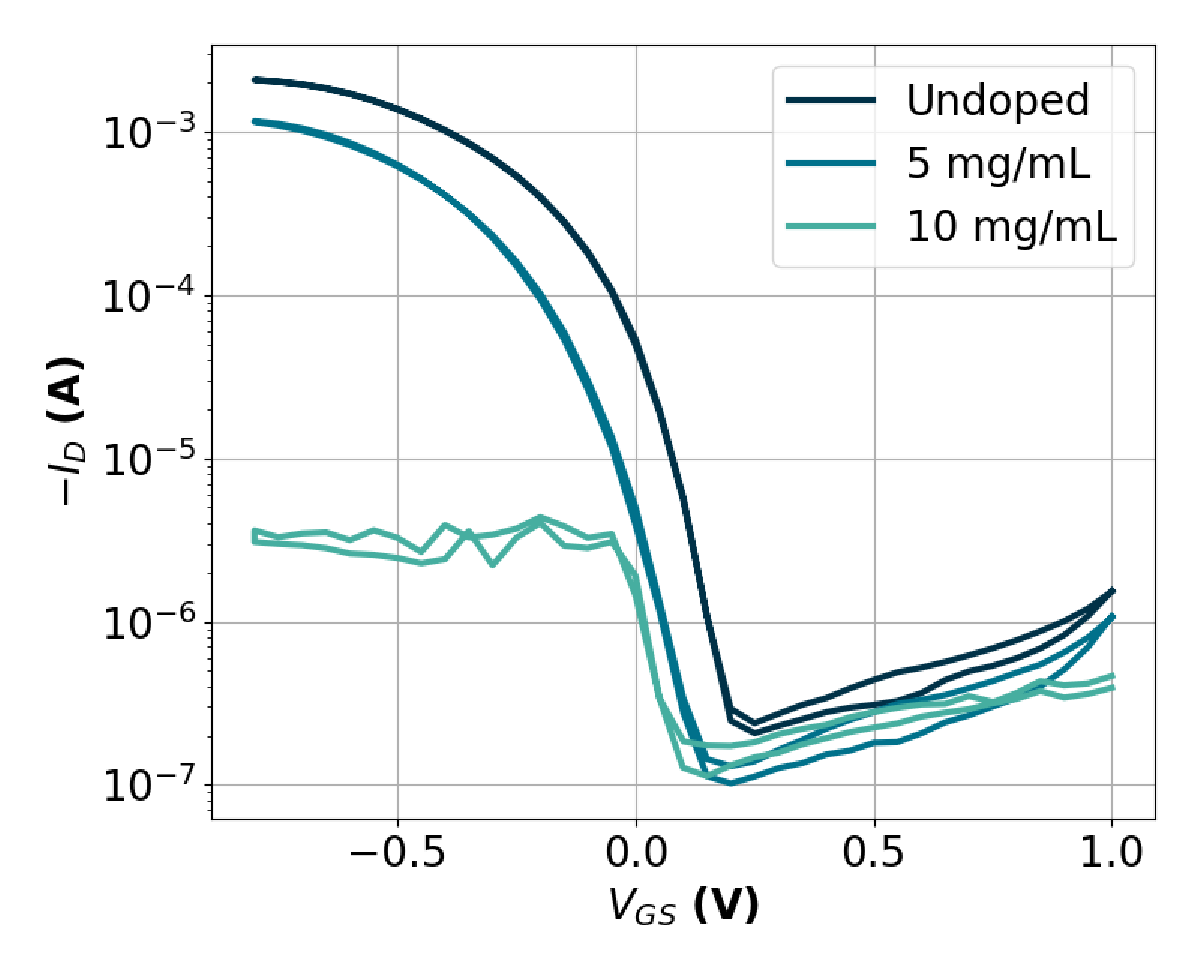
\includegraphics[width=5.5cm]{Images/pdf/Shift_Vds7.pdf} }}
    \caption[Transfer characteristics comparing different doping levels]{Transfer characteristics comparing undoped, 5 mg/mL and 10 mg/mL dopants devices, each graph represent a different $V_{DS}$}
    \label{fig:shift1}
\end{figure}

Additionally, threshold values showed lower variability among different values of $V_{DS}$ with higher doping level (Figure \ref{fig:vth_vds}). In the undoped species, the variability could be caused by ORR which should be different at different drain biased conditions. Whereas, in the doped species this variability should decrease since we are reducing ORR when doping by depleting reactive electrons from p(g3T2-T) with F$_{4}$TCNQ, hence assuring a better stability in air \cite{tanTuningOrganicElectrochemical2022}. %Further analysis needs to be done to confirm this hypothesis.  %Then although we are impacting mobility and repeatability among loops, the values at different drain biased are maintain. 

\begin{figure}[ht]
  \centering
  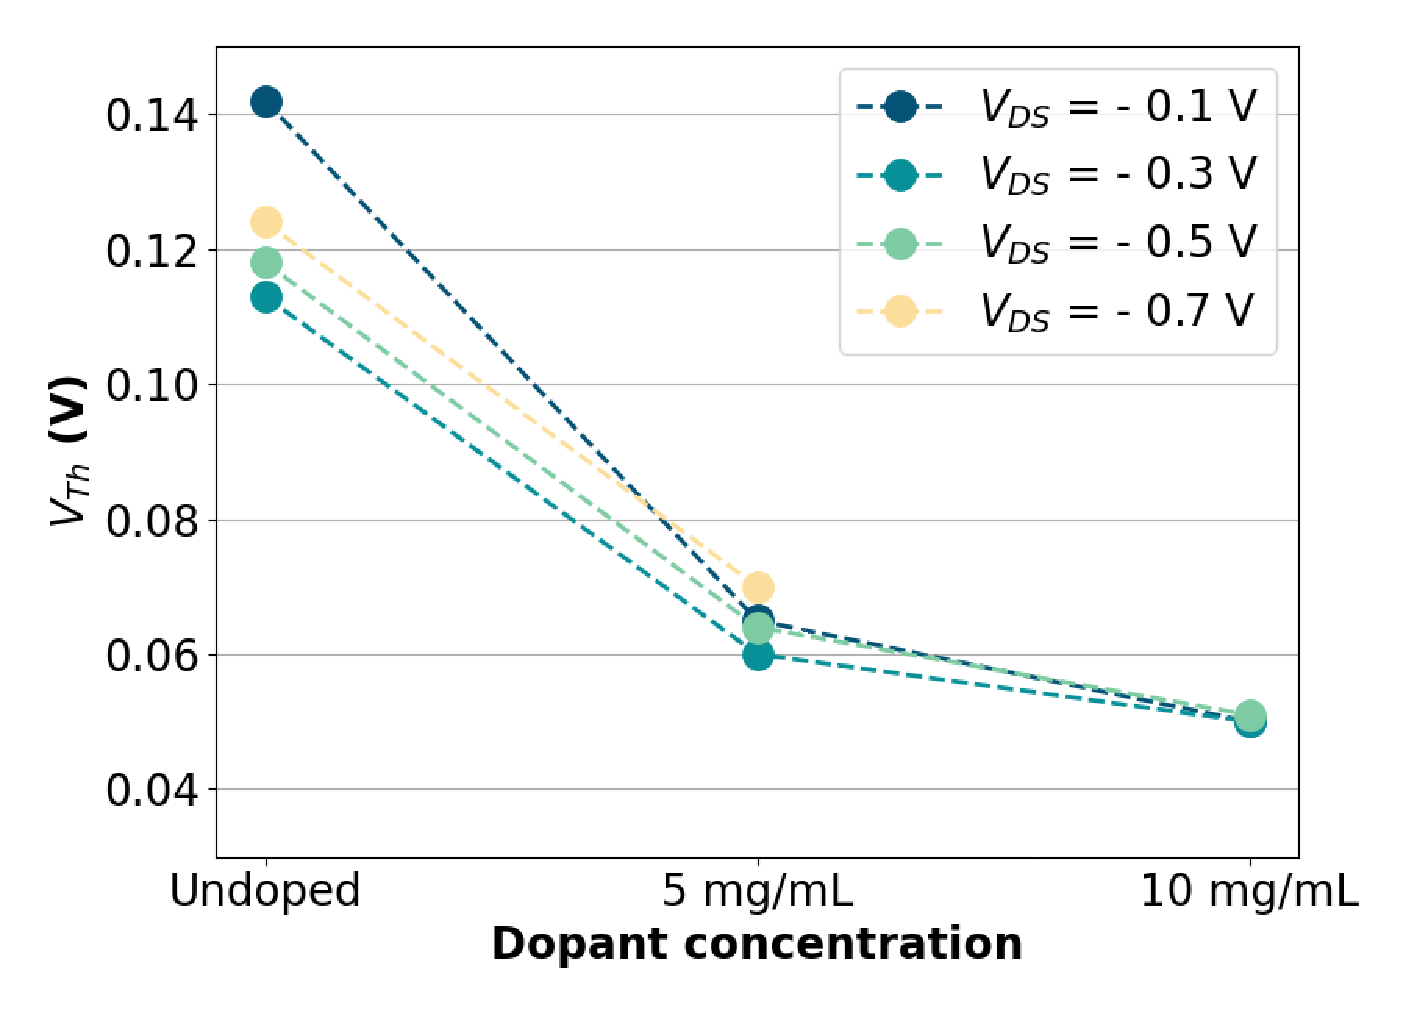
\includegraphics[width=8cm]{Images/pdf/vth_shift_vds.pdf}
  \caption[Threshold shift at different doping levels and $V_{DS}$]{Threshold shift at different doping levels and $V_{DS}$, calculations were done using data shown in Figure \ref{fig:transx2}.}
  \label{fig:vth_vds}
\end{figure}

Moreover, something that it is not shown in this report but it was perceived during analysis, there is higher repeatability of transfer characteristics with undoped OECT devices. The saturation of ORR in undoped species, as stated before, may maintain repeatability. However, variability in doped species needs yet to be further study. %Potential for appendix
%but it is yet unclear. %An new hypothesis that could explained is to consider our environmental conditions as a infinite reservoir of molecular oxygen, until this unwanted doping and ORR reaches saturation, making it stable. In the case of F$_{4}$TCNQ, stability is still unclear and further investigation will be done in the next sections.

\subsection{Stability on Air of p(g3T2-T)}
Channel conductivity of an undoped device was measured immediately after spin-coating exhibiting a value of 1 $\mu$S, after the patterning process described in previous sections, the conductivity increased three orders of magnitude yielding to approximate 1 mS. Although, $\mu$S values already represent a sign of oxidation, the patterning process oxidizes our material even more. %In this section, a way to revert this oxidation and find a compatible process to obtain accumulation-mode OECTs.
%Before getting into the revers

Measurements of $I_{D}$ at -0.3 V of $V_{DS}$ and no gate-biased exhibited a small decrease of 4\%, and small increase of 15\% within two hours in in $N_{2}$ and air environment, respectively. Air stability is seeing after patterning but due to the unwanted doping.

Same study was performed with a doped device with 5 mg/mL of F$_{6}TCNQ$ dopant, obtaining a higher level of doping than using F$_{4}TCNQ$, as it can be examined in Appendix A. The channel conductivity yielded to a value of 266 $\mu$S with a reduction of 1.2\% within one hour in $N_{2}$ environment, and same value with minimal fluctuation of 1.0\% within one hour in ambient condition. Showing a lower conductivity compared to the oxidized p(g3T2-T) but same stability in air, as stated in reference \cite{tanTuningOrganicElectrochemical2022}.

Interestingly, upon contact with SSE precursor, conductivity of both samples drops significantly, around six orders of magnitude, under $N_{2}$ environment, basically until reaching the sensitivity limits of our equipment, and noisy signal is perceived, as shown in Figure \ref{fig:revox1}A. Our first hypothetical explanation relates to the fact that p(g3T2-T), as a type VI OMIEC, has no chemical binding with $TCNQ^{-}$ anions. Upon contact with the electrolyte, anions are dragged to itself rather than staying in the backbone of the polymer (de-doping), leading to its original insulating state, which is required for accumulation-mode OECTs.
%\begin{table}[ht]
%\centering
%\caption{Conductivity measurements of undoped p(g3T2-T)}
%\begin{tabular}{l|c}
%Condition  & Conductivity (S) \\\hline
%Unpatterned & 1.3 $\times$ 10^{-6} \\
%Patterned & 1.0 $\times$ 10^{-3} \\
%\end{tabular}
%\label{tab:cond}
%\end{table}

\begin{figure}[ht]
    \centering
    \subfloat[]{{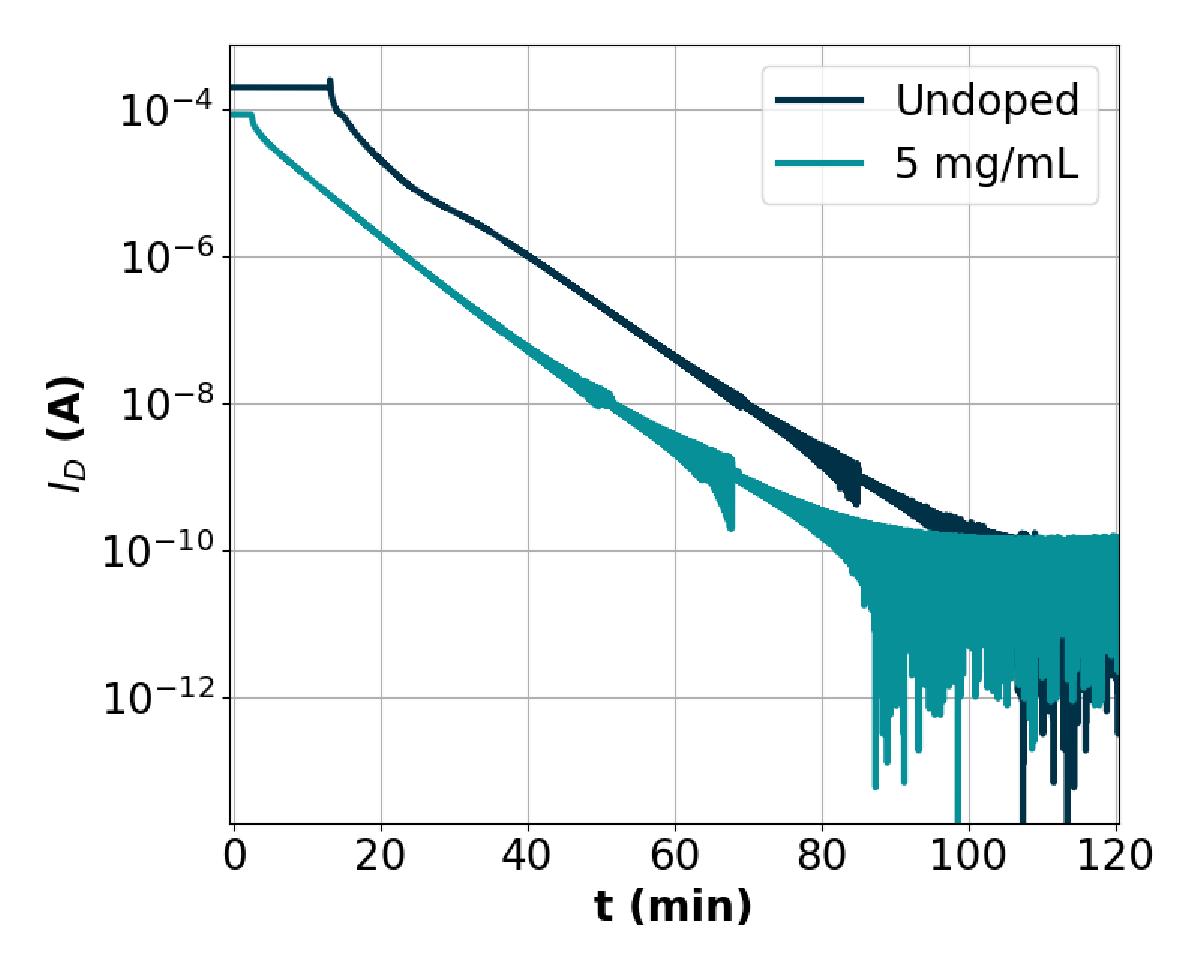
\includegraphics[width=6cm]{Images/pdf/revox_gb_only.pdf} }}
    %\qquad
    \subfloat[]{{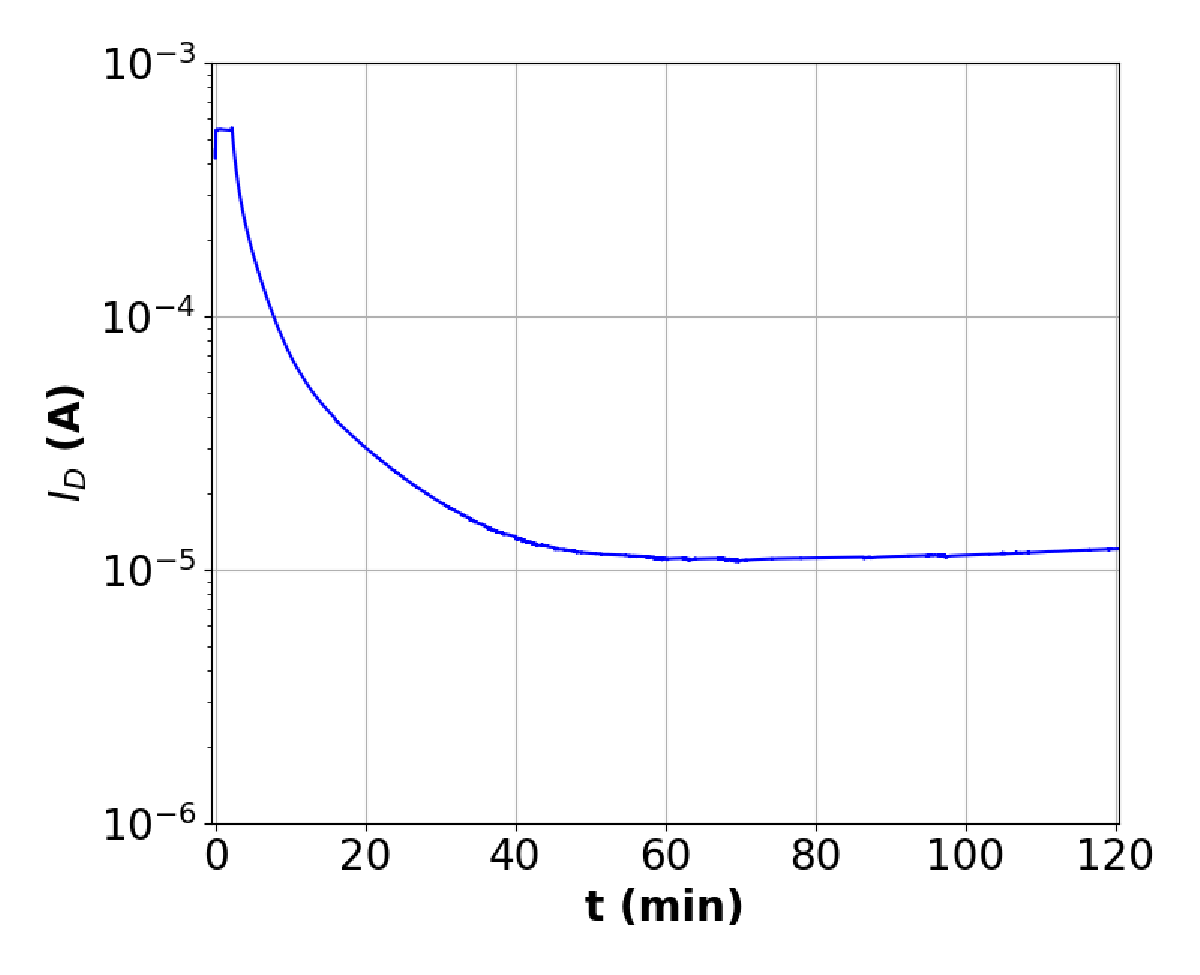
\includegraphics[width=6cm]{Images/pdf/revox_air.pdf} }}
    %\subfloat[Ambient and $N_{2}$ environment]{{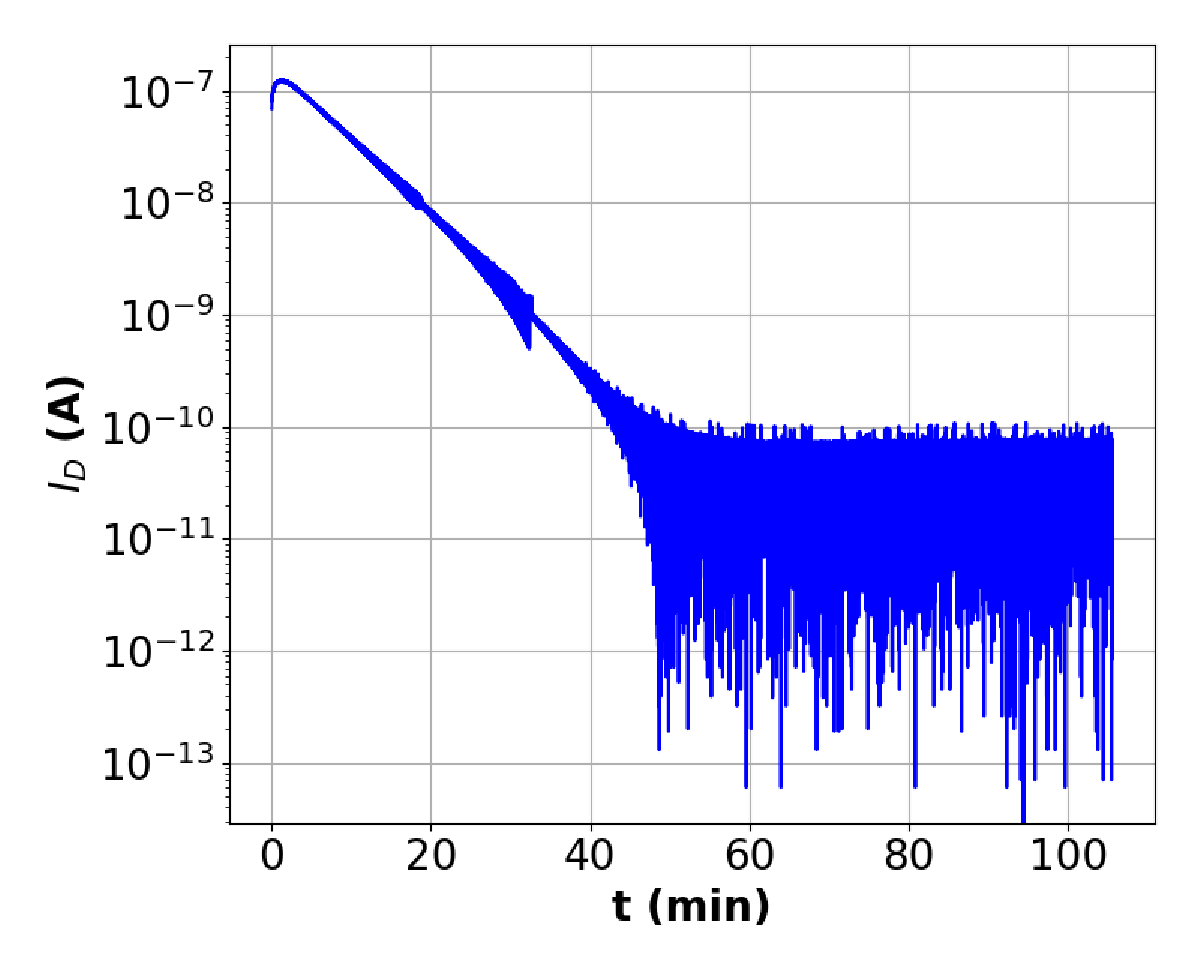
\includegraphics[height=5.5cm]{Images/pdf/revox_gb_afterair.pdf} }}
    \caption[Drain current over time of undoped-p(g3T2-T) coupled with SSE precursor]{Drain current over time of undoped p(g3T2-T) coupled with SSE precursor under A) $N_{2}$, and B) ambient environment%, C)$N_{2}$ environment after B)
    .}
    \label{fig:revox1}
\end{figure}

On the other hand, as seen in Figure \ref{fig:revox1}B, under ambient conditions, there is a smaller decrease of more than one order of magnitude for the undoped sample. The doped sample show a similar and faster drop in the first 15 minutes, but then a sudden increase of $I_{D}$ is perceived. In both scenarios, ORR prevents a higher decrease of current, and the fluctuation seen in the doped species may be due the simultaneous ORR and the de-doping, as commented before. %Another undoped sample share the same results.

\begin{figure}[ht]
    \centering
    %\subfloat[N$_{2}$ environment]{{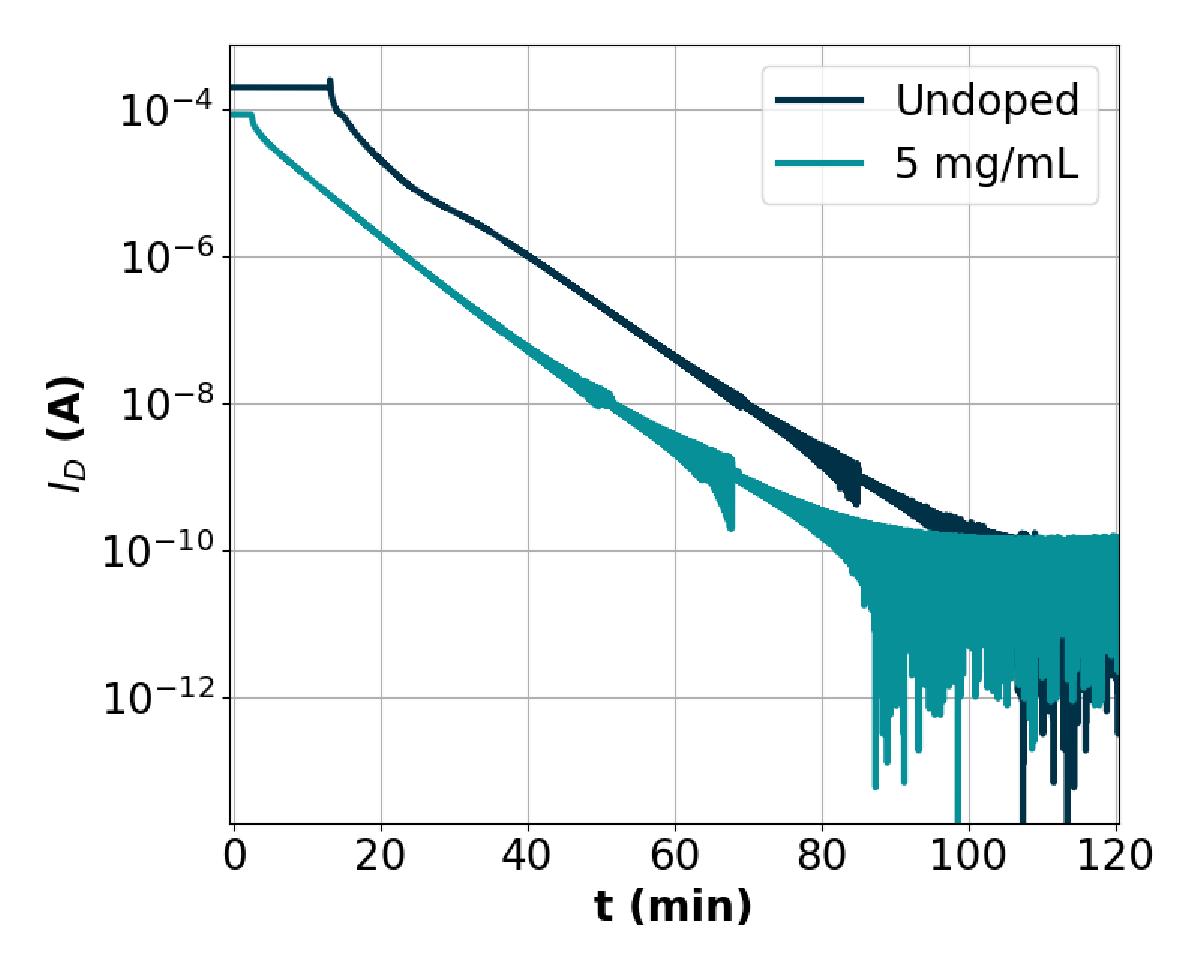
\includegraphics[height=5.5cm]{Images/pdf/revox_gb_only.pdf} }}
    %\subfloat[Transfer in ambient]{{
    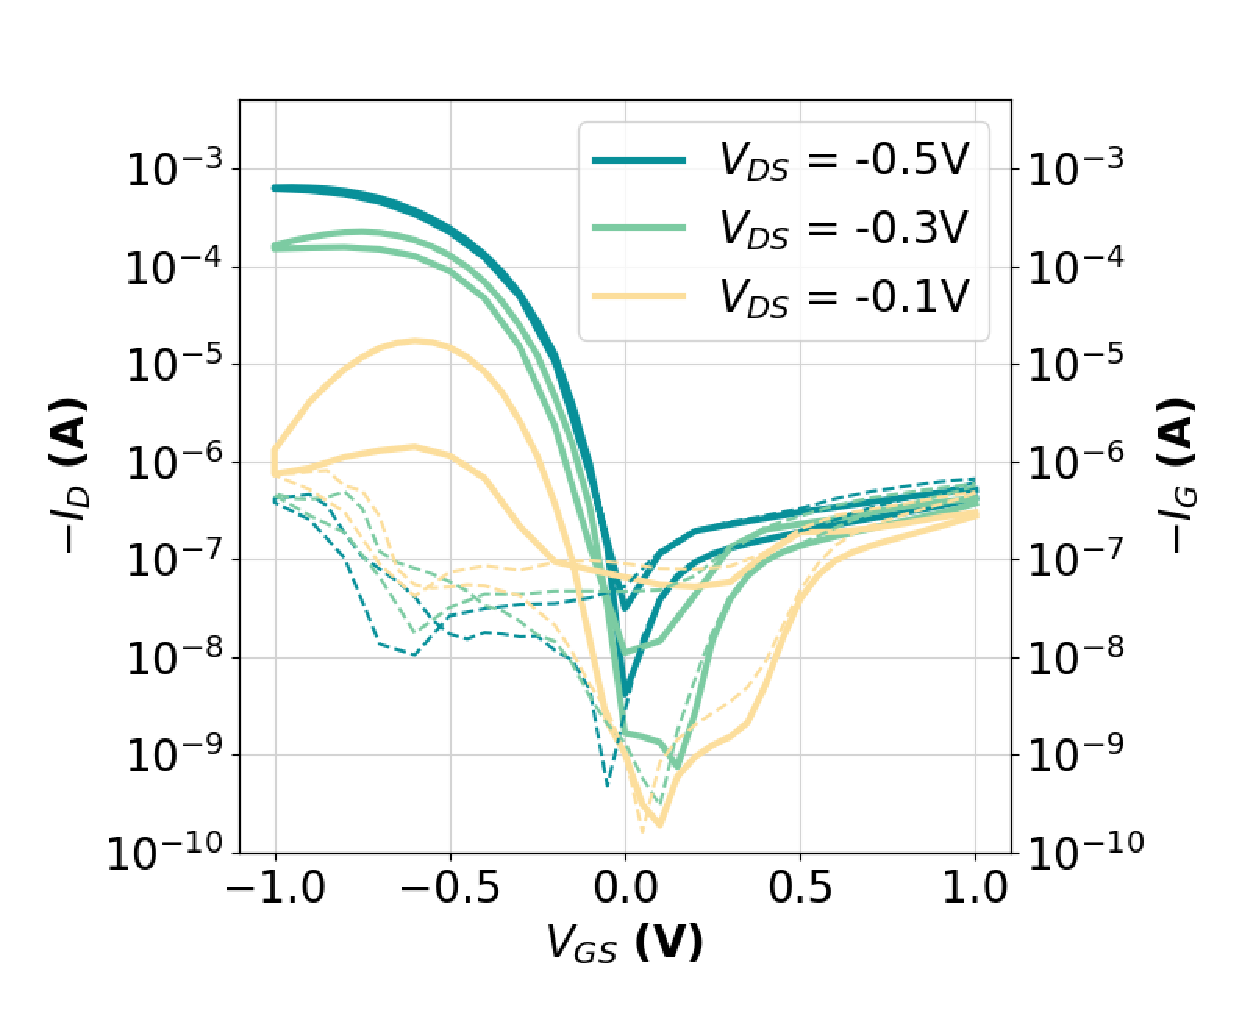
\includegraphics[height=6cm]{Images/pdf/revox_transfer_loop2.pdf}% }}
    \caption[Transfer characteristics after dedoping]{Transfer characteristics at different $V_{DS}$ under ambient conditions}
    \label{fig:transrevox1}
\end{figure}

Transfer curves of the undoped device using an Ag/AgCl pellet as gate were measured under ambient conditions after de-doping in $N_{2}$ environment. The device had an ON voltage very close to zero, as seen in Figure \ref{fig:transrevox1}, even shifting to negative values as runs were progressing. Although, there a clear sign of degradation of the device. 

The de-doping could become a method to obtain an accumulation-mode OECTs by reversing the oxidation of p(g3T2-T).

\subsection{Reverse Oxidation of Undoped-p(g3T2-T)}
From the previous section, the de-doping of the p(g3T2-T) took around two hours to obtain a fully insulating state. However, we could speed up this process by positive-biased the gate of our already patterned oxidized sample. 

Additionaly, another method acknowledge by Biosens group members is going to be tested, using high temperature to revert the oxidation of an OECT device.  

\subsubsection{By Electrochemical Dedoping}
A +1V gate biased was applied 

\begin{figure}[ht]
    \centering
    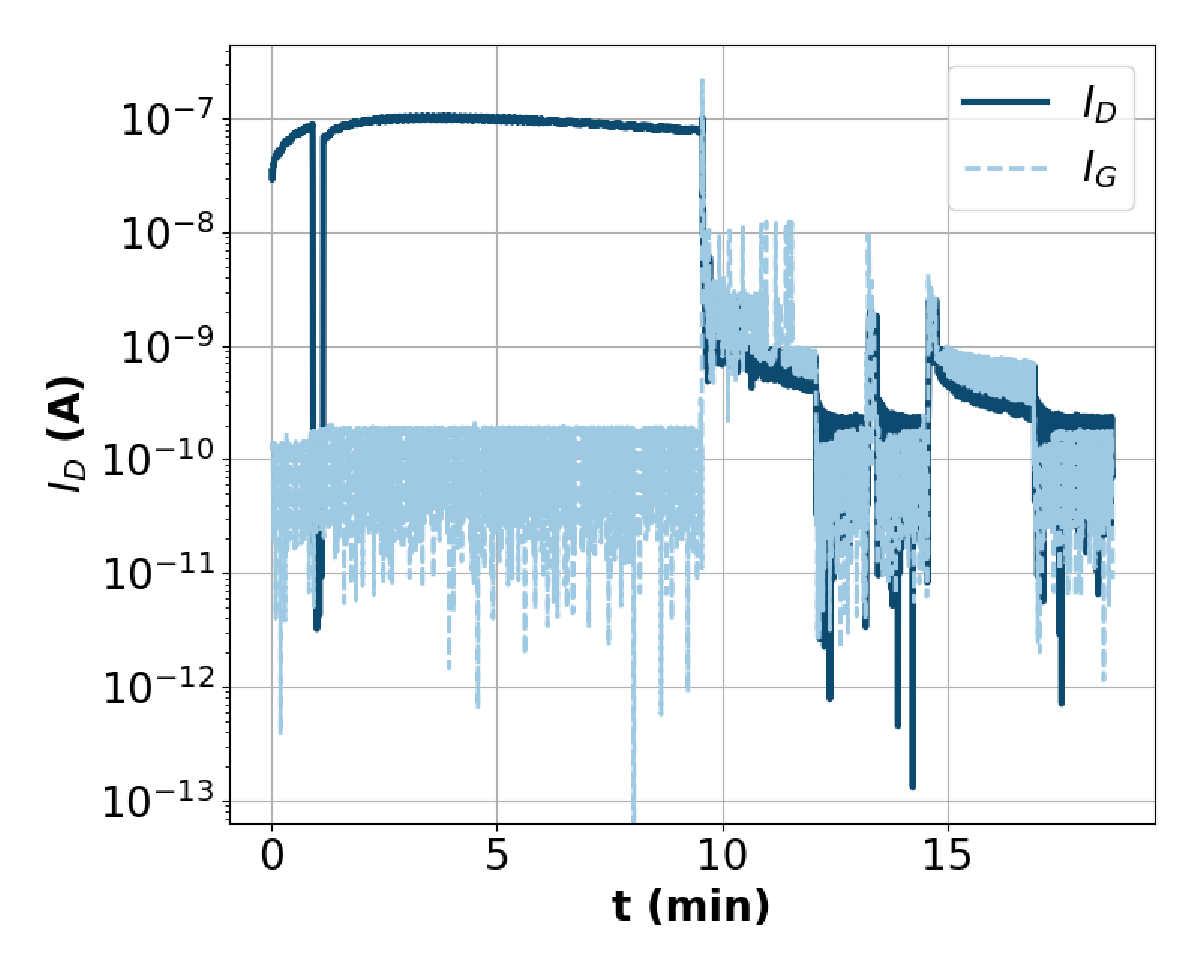
\includegraphics[height=6cm]{Images/pdf/elec-dedop1.pdf}
    \caption[Transfer characteristics after dedoping]{Transfer characteristics at different $V_{DS}$ under ambient conditions}
    \label{fig:revox2}
\end{figure}


\subsubsection{By Heating}


\subsection{Solid-OECTs using Undoped p(g3T2-T)}


%The Ag/AgCl gate electrode’s work function is reasonably constant, the work function of an OMIEC gate electrode however may vary depending on its processing history and redox reactions with other species present in the electrolyte (e.g. molecular oxygen).28 Applying VGS only determines the potential difference between the gate and channel but does not control the potentials of either electrode (hence the position of the Fermi level) with respect to a reference. This leads to many challenges in operating an OECT with OMIEC gate electrodes.


\subsubsection{Dropcasted Solid-State Electrolyte}

\subsubsection{OECT with Dropcast Solid-State Electrolyte}

\subsubsection{OECT with Photopatternable Solid-State Electrolyte}

\subsubsection{OECT with Inkjet-Printed Solid-State Electrolyte}


\subsection{Solid-OECTs using Doped-p(g3T2-T)}



%Achieving effective charge transfer between the analyte and OMIEC requires appropriate alignment of the electrochemical potential of electrons on the OMIEC electrode and the redox specie. Failure to do so may result in the subsequent transfer of charges to other redox-active sinks in the environment, leading to undesirable side reactions and products that may interfere with the OMIEC’s operation. Electrons flow from a region of higher to lower electrochemical potential. Hence, achieving electron transfer from redox-active species to the OMIEC requires the latter to have a deep LUMO (high electron affinity) \cite{tanMixedIonicElectronic2022} %paper

%\section{Conclusion}
%\lipsum[86-88]

%%% Local Variables: 
%%% mode: latex
%%% TeX-master: "thesis"
%%% End: 
